\chapter{Clustering Jerárquico}
\label{chapter:jerarquico}

Como se mencionó en el capítulo anterior las galaxias tienen sus componentes en una estructura jerárquicamente organizada, donde el núcleo está contenido dentro del Esferoide y el Disco Fino dentro del grueso. A modo de ejemplo puede observarse en la Fig~\ref{fig:mwschema} una vista esquemática de cómo se cree que es la forma de nuestra Vía láctea y se puede apreciar esta jerarquía.

\begin{figure}
    \centering
    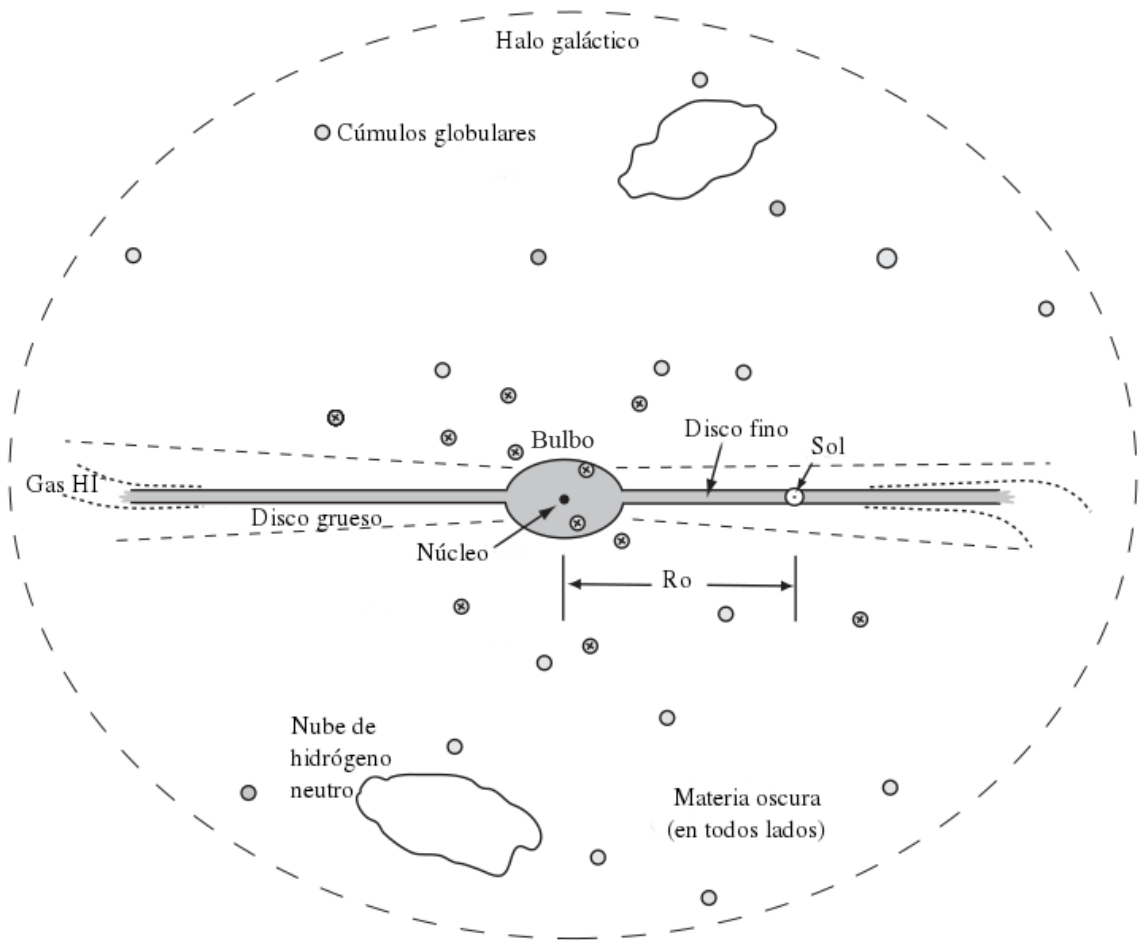
\includegraphics[width=.9\textwidth]{clustering jerarquico/figures/mwschema.png}
    \caption{\label{fig:mwschema} Vista esquemática de canto de la Vía Láctea \citep{sparke2007galaxies}}
\end{figure}

En minería de datos, el \gls{HC} se refiere a una familia de algoritmos que buscan en los datos grupos organizados jerárquicamente. Así, a medida que se aumenten la cantidad de clusters buscados, estos se irán dividiendo o fusionando hasta alcanzar el número deseado dependiendo del tipo del algoritmo utilizado, como se explicará a continuación.

Para usar este enfoque es necesario sospechar que los datos tienen algún tipo de estructura con diferentes niveles de granularidad o resolución, como es el caso de las componentes de una galaxia \citep{hubble1936realm}.

En la práctica la forma de generar esta jerarquía puede realizarse de dos maneras distintas

\begin{itemize}
    \item \textbf{Aglomerativas}: Este es un acercamiento ascendente. Cada observación comienza en su propio grupo, y los pares de grupos son mezclados mientras uno sube en la jerarquía.
    \item \textbf{Divisivas}: Este es un acercamiento descendente. Todas las observaciones comienzan en un grupo, y se realizan divisiones mientras uno baja en la jerarquía.
\end{itemize}

Para poder decidir qué grupos deberían ser combinados (para métodos aglomerativos), o cuando un grupo debería ser dividido (para métodos divisivos), se requiere una medida de disimilitud entre conjuntos de observaciones. En la mayoría de los métodos de \gls{HC}, esto es logrado mediante el uso de una medida específica de distancia entre grupos de observaciones, también llamado ``\textit{linkage}'', que especifica la disimilitud de conjuntos como una función de las distancias dos a dos entre ciertas observaciones en los conjuntos \citep{sharma2019comparative}.

En este trabajo utilizaremos la implementación de \gls{HC} aglomerativo provista por scikit-learn \citep{scikit-learn}, la distancia euclidiana para medir la distancia entre puntos, y los  linkages descritos a continuación:

\begin{itemize}
    \item \textbf{Ward}: Minimiza la suma de las diferencias al cuadrado dentro de todos los clusters. Es un enfoque de minimización de la varianza.
    \item \textbf{Complete}: Minimiza la distancia máxima entre observaciones de pares de clusters.
    \item \textbf{Average}: Minimiza la media de las distancias entre todas las observaciones de pares de conglomerados.
    \item \textbf{Single}: Minimiza la distancia entre las observaciones más cercanas de pares de conglomerados.
\end{itemize}

Optamos por utilizar \gls{HC} aglomerativo ya que parece ser el que mejores resultados da en el área de estudio \citep{yu2022hierarchical}. En cuanto a la distancia euclidiana, esta fue elegida dado que los dominios de los datos con los cuales trabajamos son continuos \citep{pillepich2018simulating}.

Por otro lado, para decidir sobre el linkage a utilizar realizamos los experimentos descriptos en la siguiente sección.

\section{Selección de linkage}

Para poder concluir en el linkage que nos da mejores resultados procedimos a aplicar \gls{HC} con todos los linkages y compararlos con el método de Abadi, sobre un conjunto de 9 galaxias. 

\begin{figure}
    \centering
    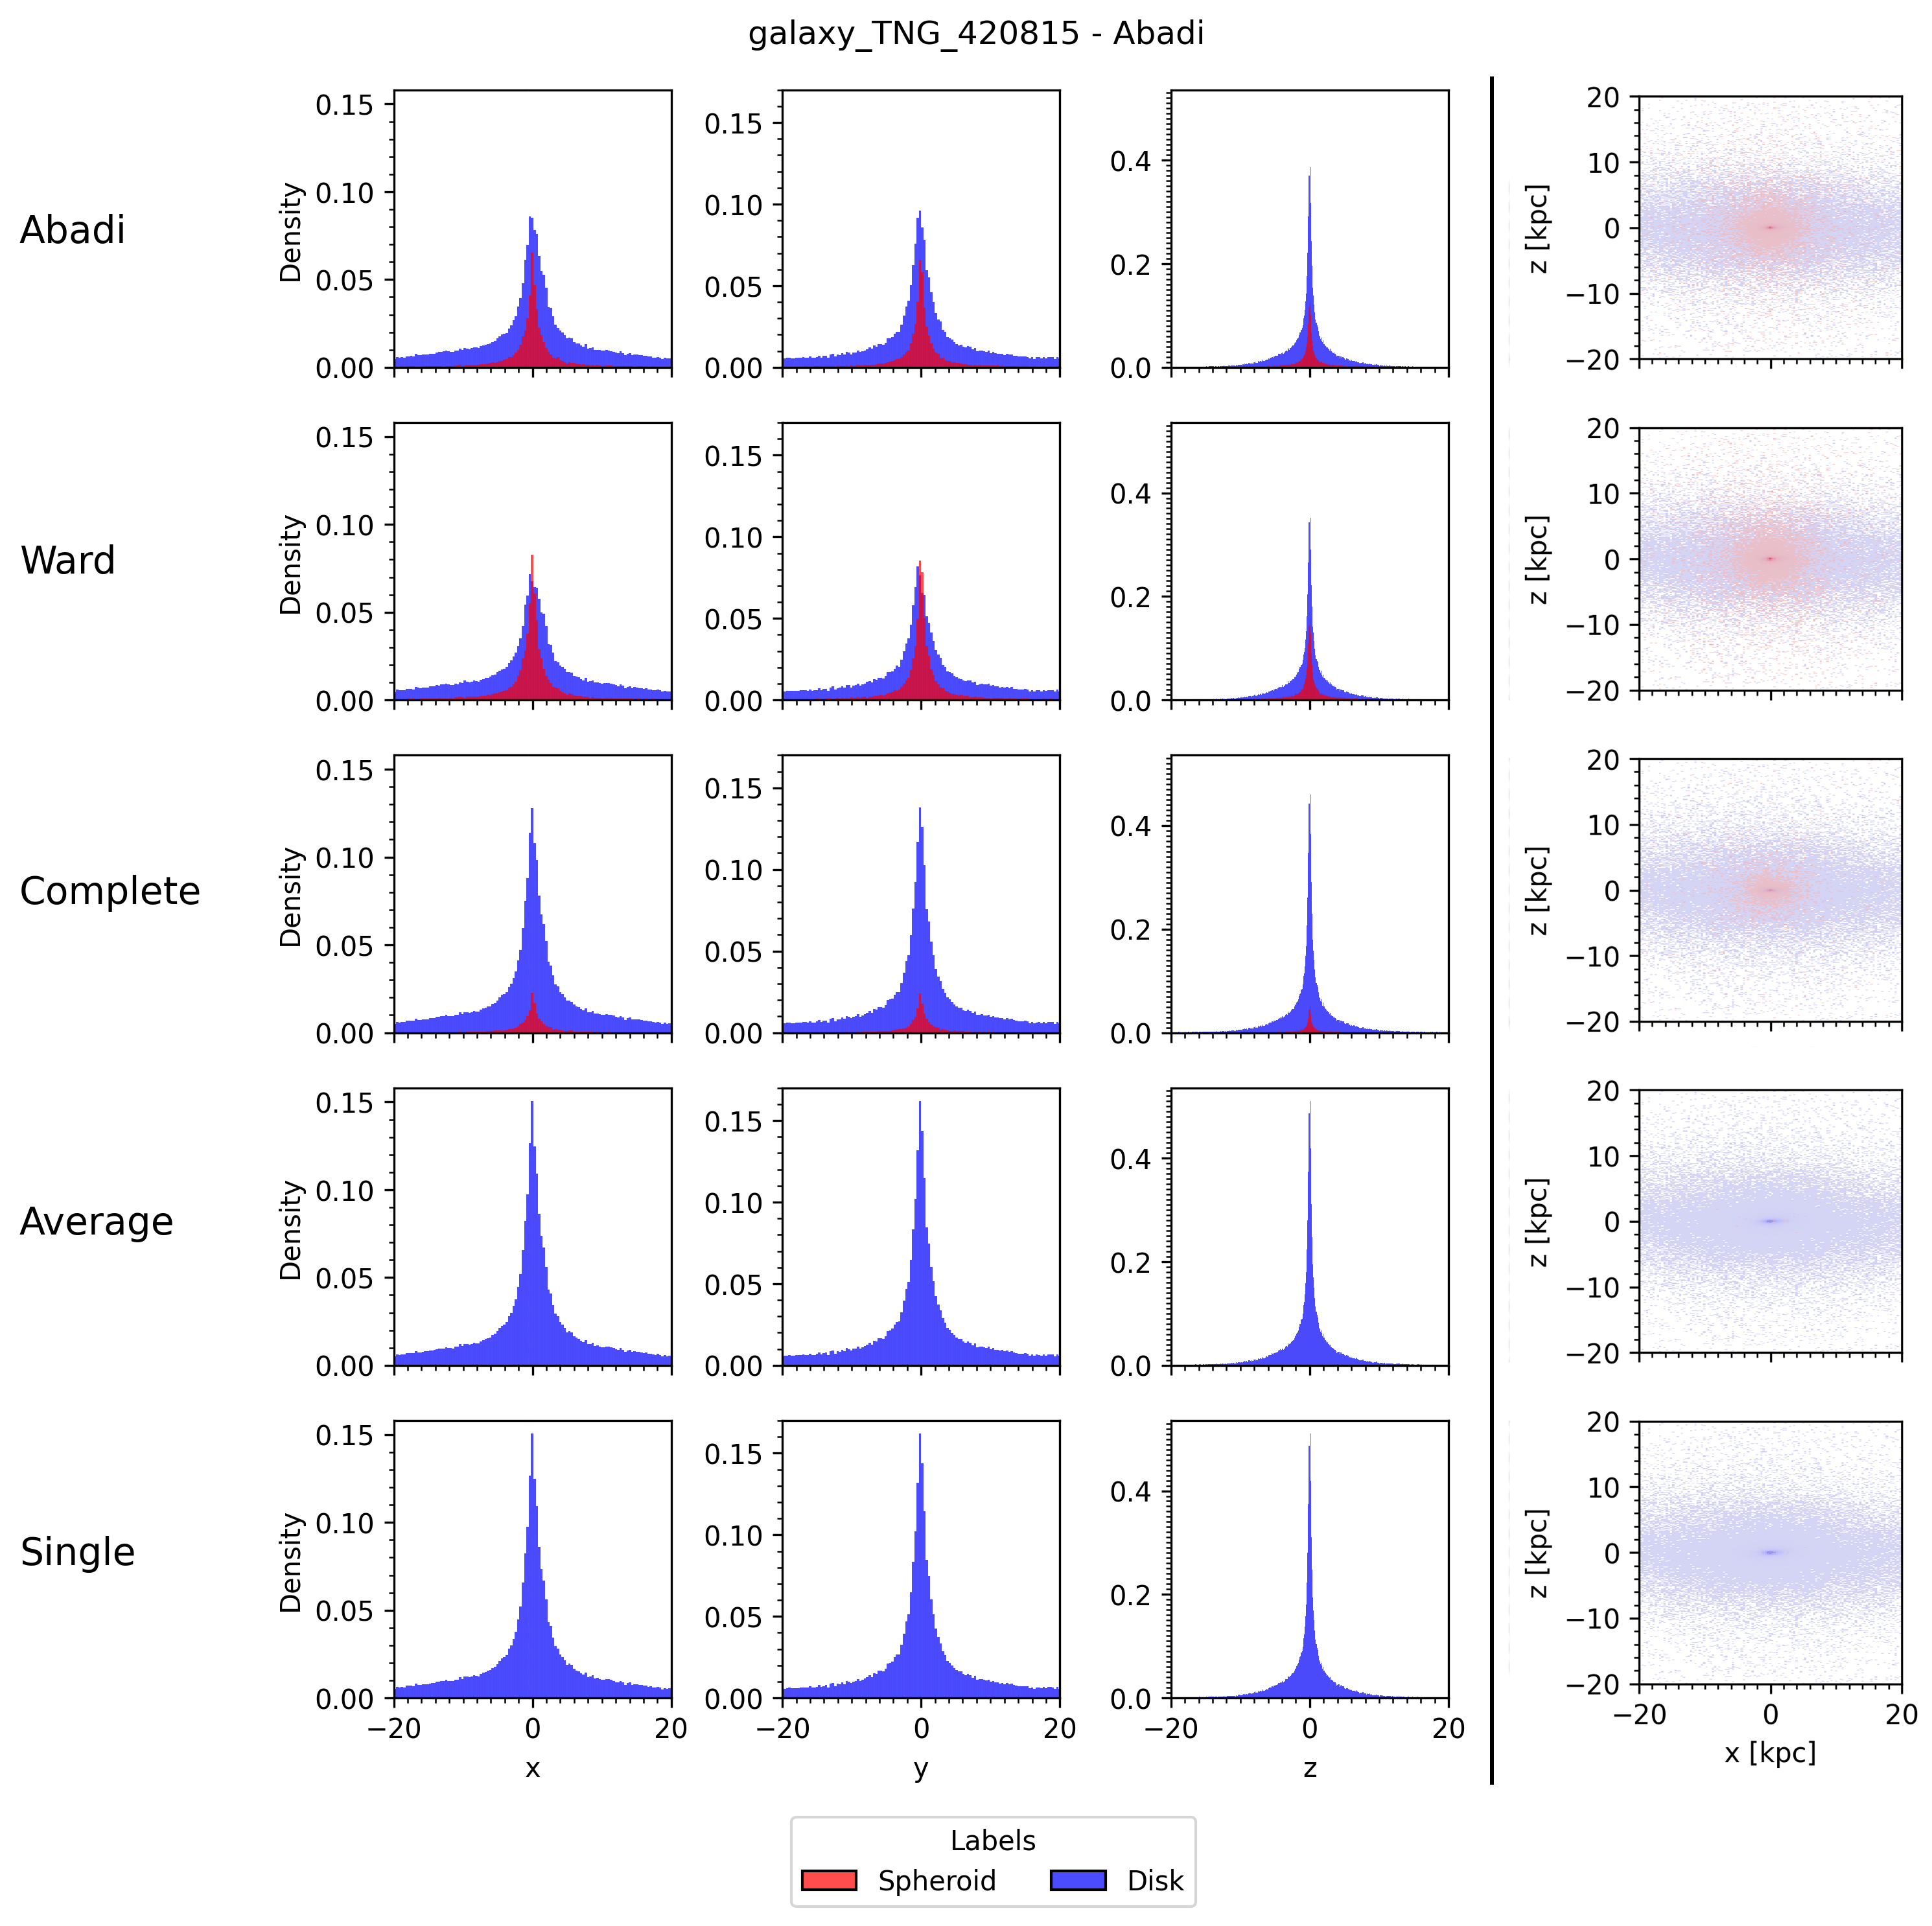
\includegraphics[width=.9\textwidth]{clustering jerarquico/figures/linkage_comparison.png}
    \caption{\label{fig:linkage_comparison} Histograma comparando los grupos obtenidos con \gls{HC} con diferentes linkages contra Abadi sobre la galaxia \textit{galaxy\_TNG\_420815} en el espacio real. Además se incluyen histogramas comparando eje a eje los grupos obtenidos sobre el espacio real.}
\end{figure}

Como se puede observar en la Fig~\ref{fig:linkage_comparison}, utilizar los linkages Average y Single resultó en un cluster con casi todas las estrellas de la galaxia en una sola componente. Esto se debe a que las partículas estelares de diferentes componentes en el espacio circularidad están tan cercanas entre ellas (ver Fig~\ref{fig:circ-scatterplot-420815}), que la tarea de encontrar clusters en dicho espacio se ve dificultada. Por lo cual, al utilizar el linkage Single el cual hace uso de la distancia mínima inter-clusters, basta con tener un solo punto alejado del resto de nuestros datos para que éste sea identificado como un único cluster. Y en el caso de linkage Average, su tarea se ve perjudicada por el alto solapamiento de los clusters. Por otro lado con linkage Complete, si bien da algunos resultados similares a Abadi, es inestable y no logra resultados con la consistencia que logra Ward en el Apéndice~\ref{appendix}.

\begin{figure}
    \centering
    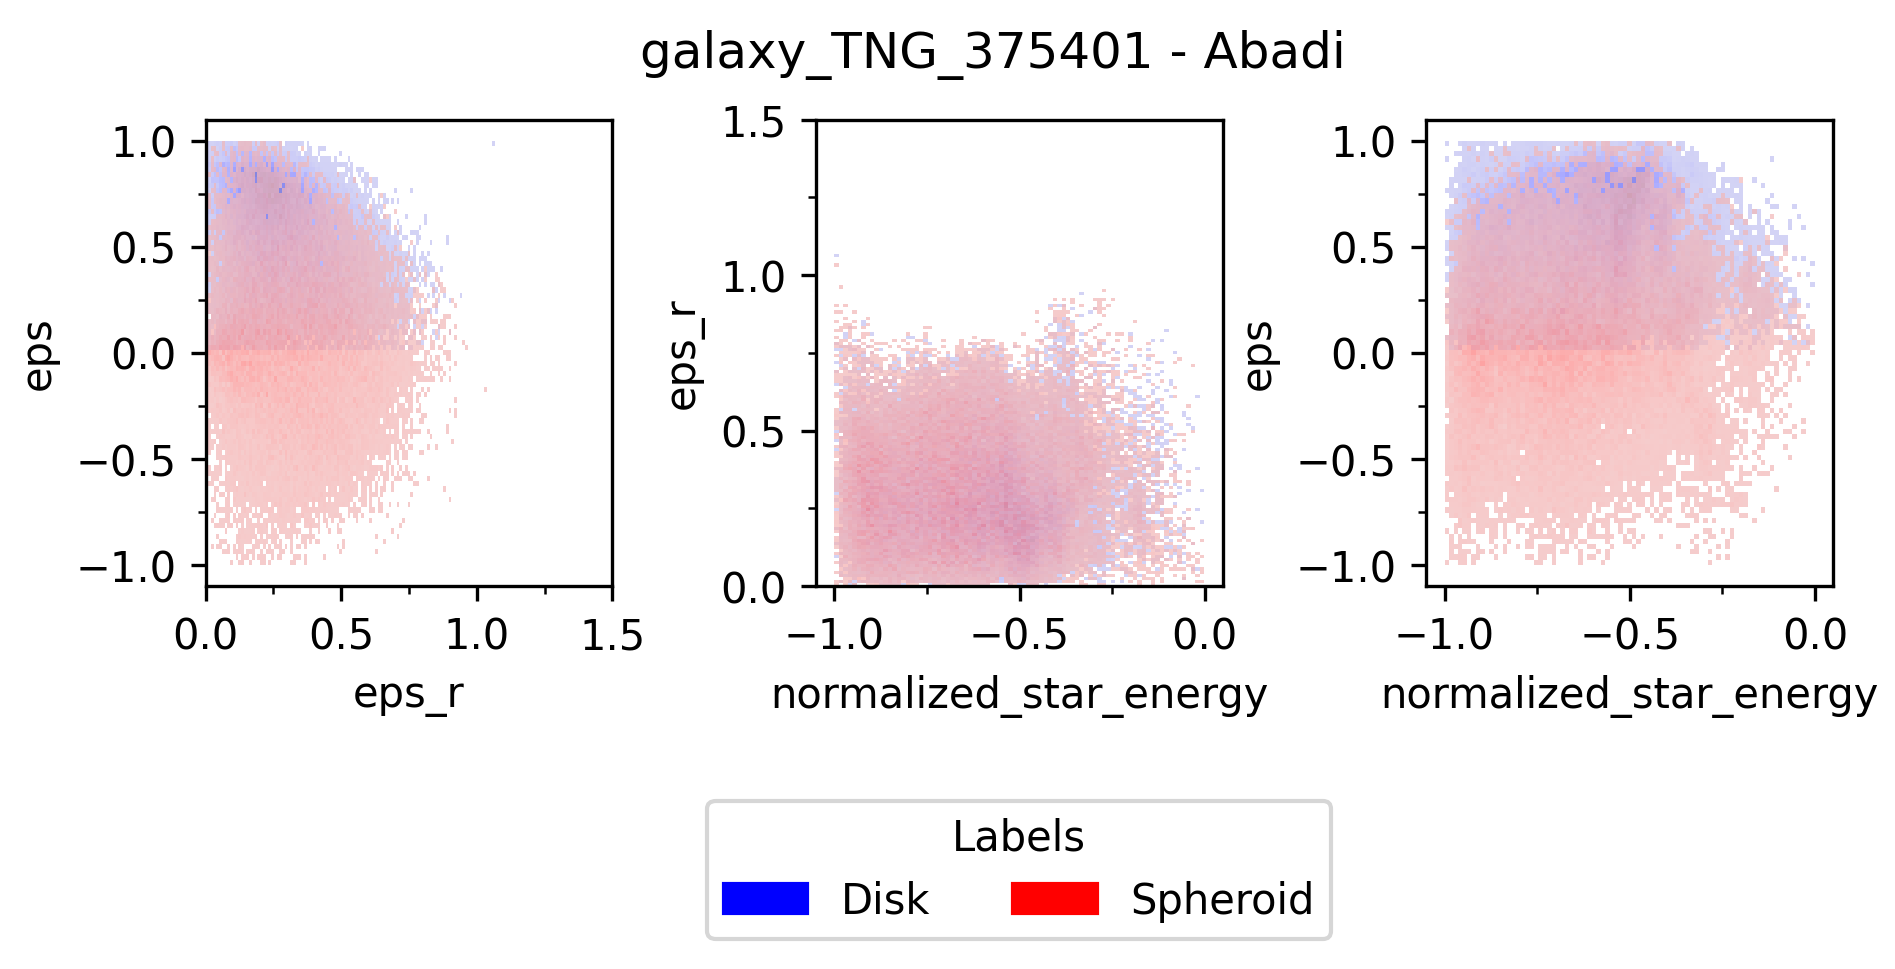
\includegraphics[width=.9\textwidth]{clustering jerarquico/figures/componentes_cercanas_circ.png}
    \caption{\label{fig:circ-scatterplot-420815} Scatterplot mostrando la cercanía de las componentes encontradas por Abadi en espacio circular sobre la galaxia \textit{TNG\_420815}.}
\end{figure}

Finalmente, los buenos resultados de Ward pueden vincularse a como la varianza de las distancia entre clusters es una métrica mucho más consistente e inmune al ruido en comparación al resto.

Puede que en datasets sin galaxias con esferoides los linkages Complete, Average y Single den mejores resultados. Pero dado que tenemos galaxias con esferoides en el dataset utilizado en este trabajo procederemos a usar solamente el linkage Ward en lo que resta del capítulo.

A partir de este momento, nos referiremos a \gls{HC} con Ward como \gls{HC} o Ward indistintamente.

\section{Detección de dos componentes: Disco y esferoide}

Antes de comenzar, es importante diferenciar como utilizaremos el término $par\acute{a}metro$ y $feature$ de aquí en adelante. Con $par\acute{a}metro$ nos referiremos a las ``variables'' que el algoritmo de aprendizaje automatizado aprende a partir de su entrenamiento, mientras que el término $feature$ será utilizado para referirse a dicha variable en nuestro conjunto de datos (es decir, una ``columna'' de los datos).

En las siguientes pruebas se procedió a utilizar \gls{HC} con los mismos features de los datos utilizados por Abadi \citep{abadi2003simulations}, $eps$, buscando 2 clusters. Los resultados obtenidos pueden observarse en la Fig~\ref{fig:2componentesCJ}. Si prestamos atención a la columna con el gráfico de $eps$ vs $normalized\_star\_energy$ se evidencia como al carecer de la heurística de Abadi, Ward no puede cortar de manera adecuada el componente disco en $normalized\_star\_energy$; esta situación hace que el esferoide sea más grande como puede verse en la Tabla~\ref{table:2componentesCJ} y afecta los perfiles de velocidades (primera columna de la Fig~\ref{fig:2componentesRotationCurve}).

\begin{figure}
    \centering
    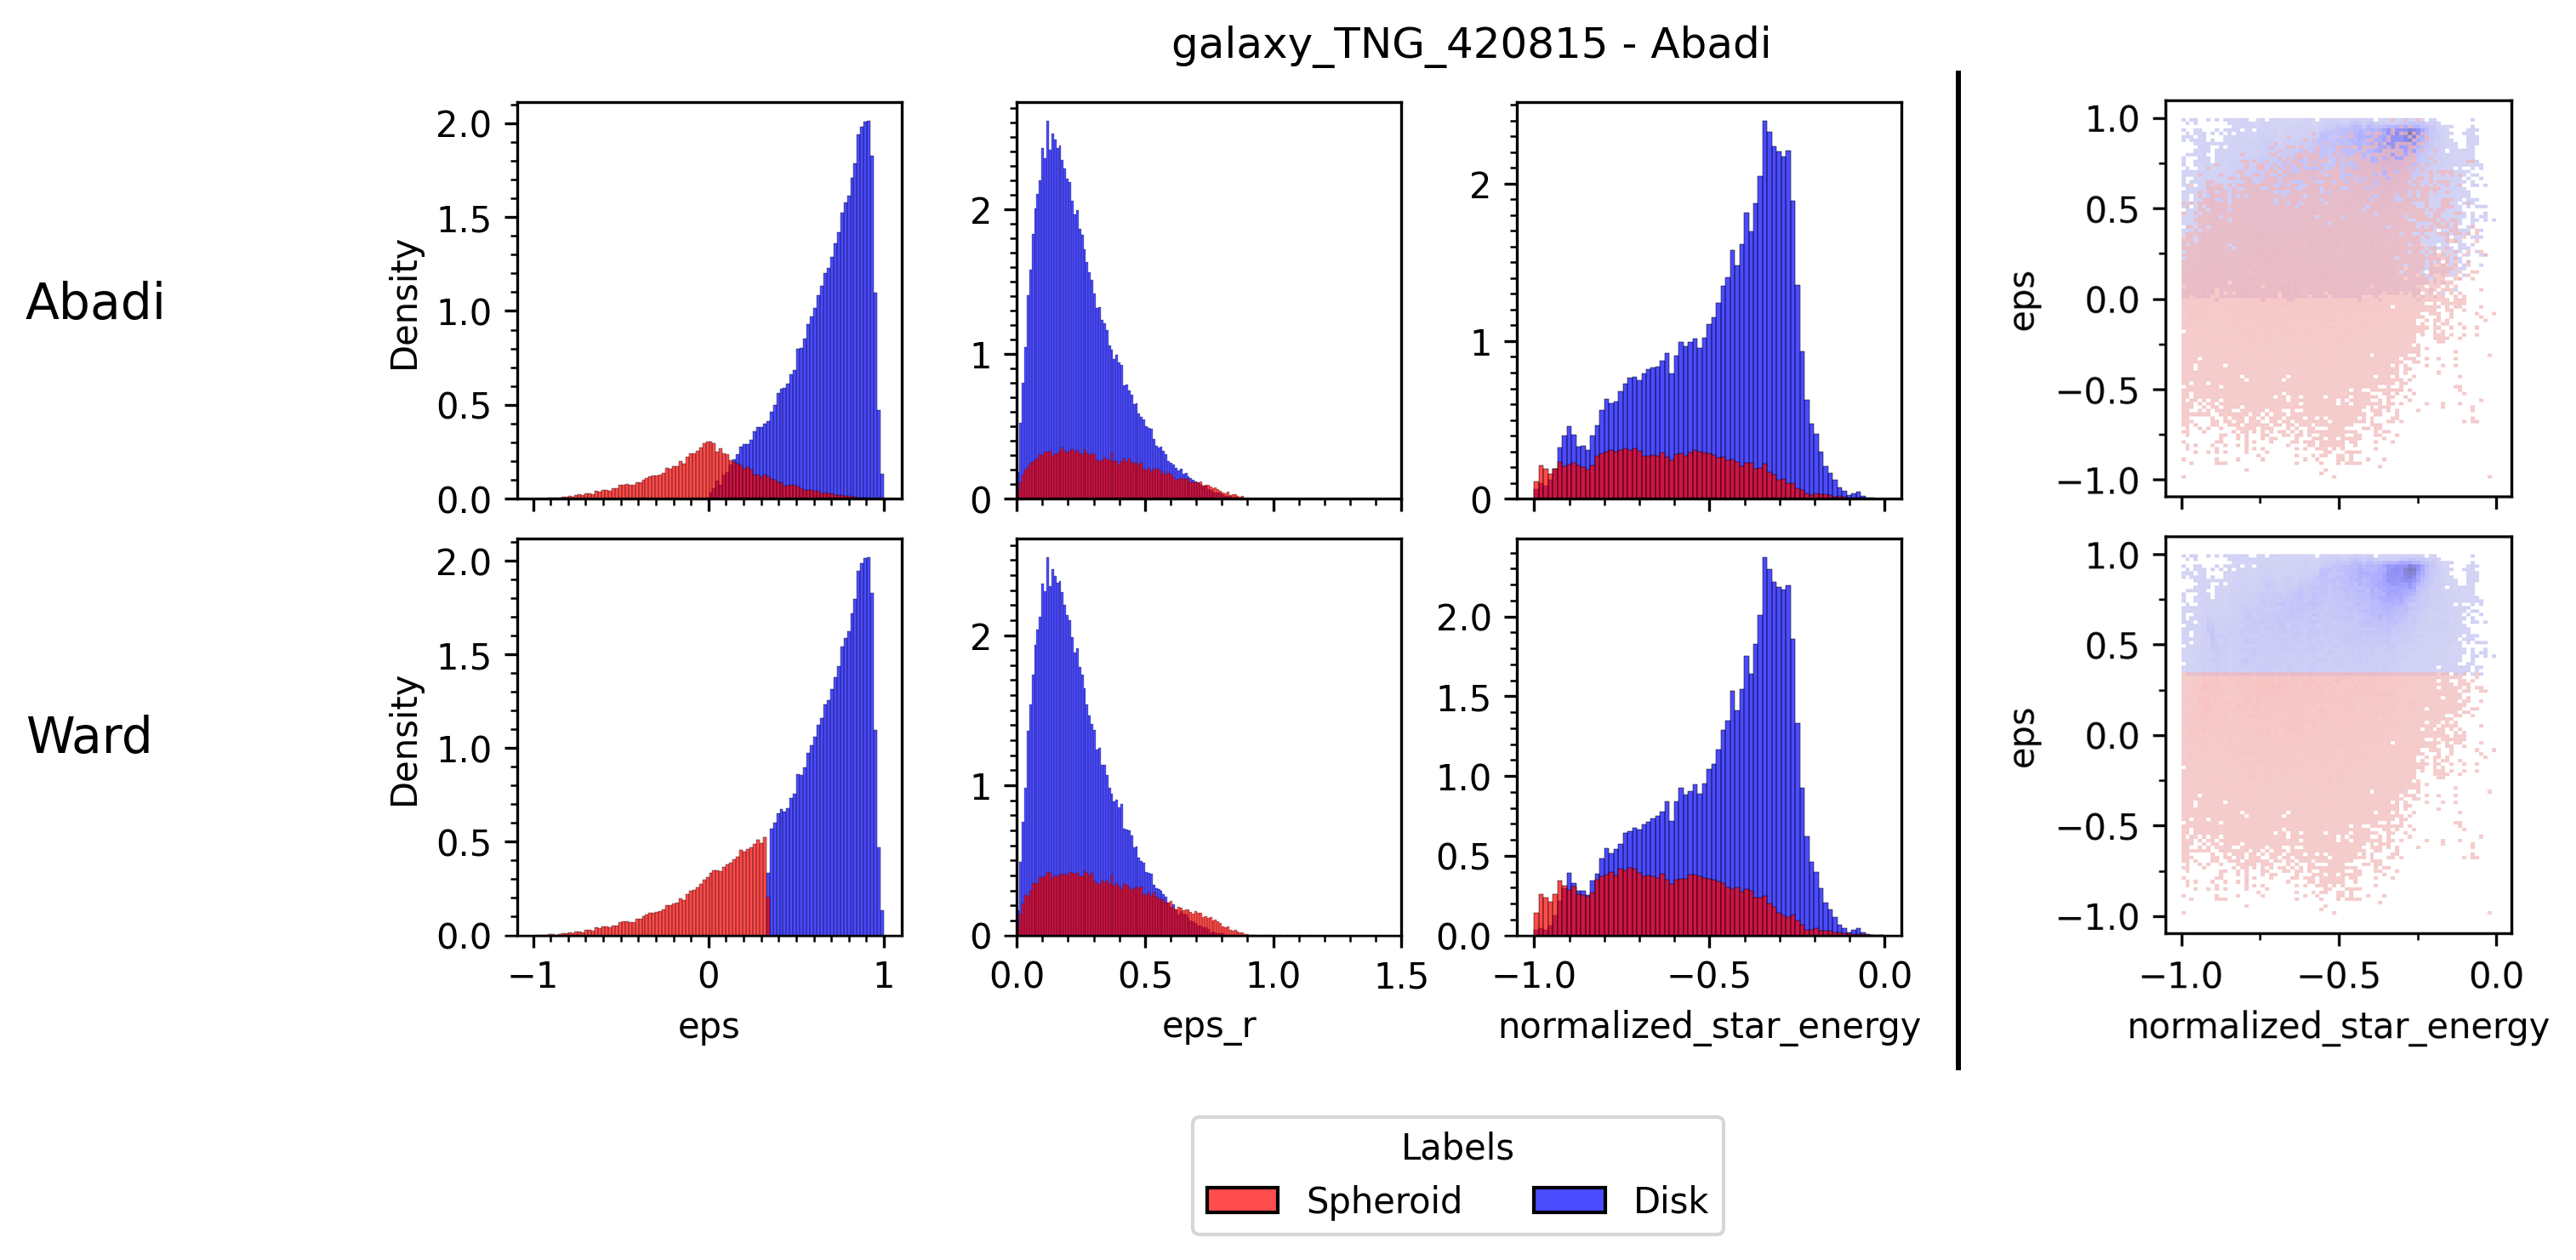
\includegraphics[width=11cm]{clustering jerarquico/figures/galaxy_TNG_420815 - abadi - base - circ histogram and scatterplot.png}
    \caption{
    \label{fig:2componentesCJ}
    Histograma y gráfico de dispersión comparando los resultados obtenidos con Abadi contra los obtenidos con \gls{HC} con linkage Ward sobre la galaxia \textit{galaxy\_TNG\_420815} en espacio circular.}
\end{figure}

\begin{figure}
    \centering
    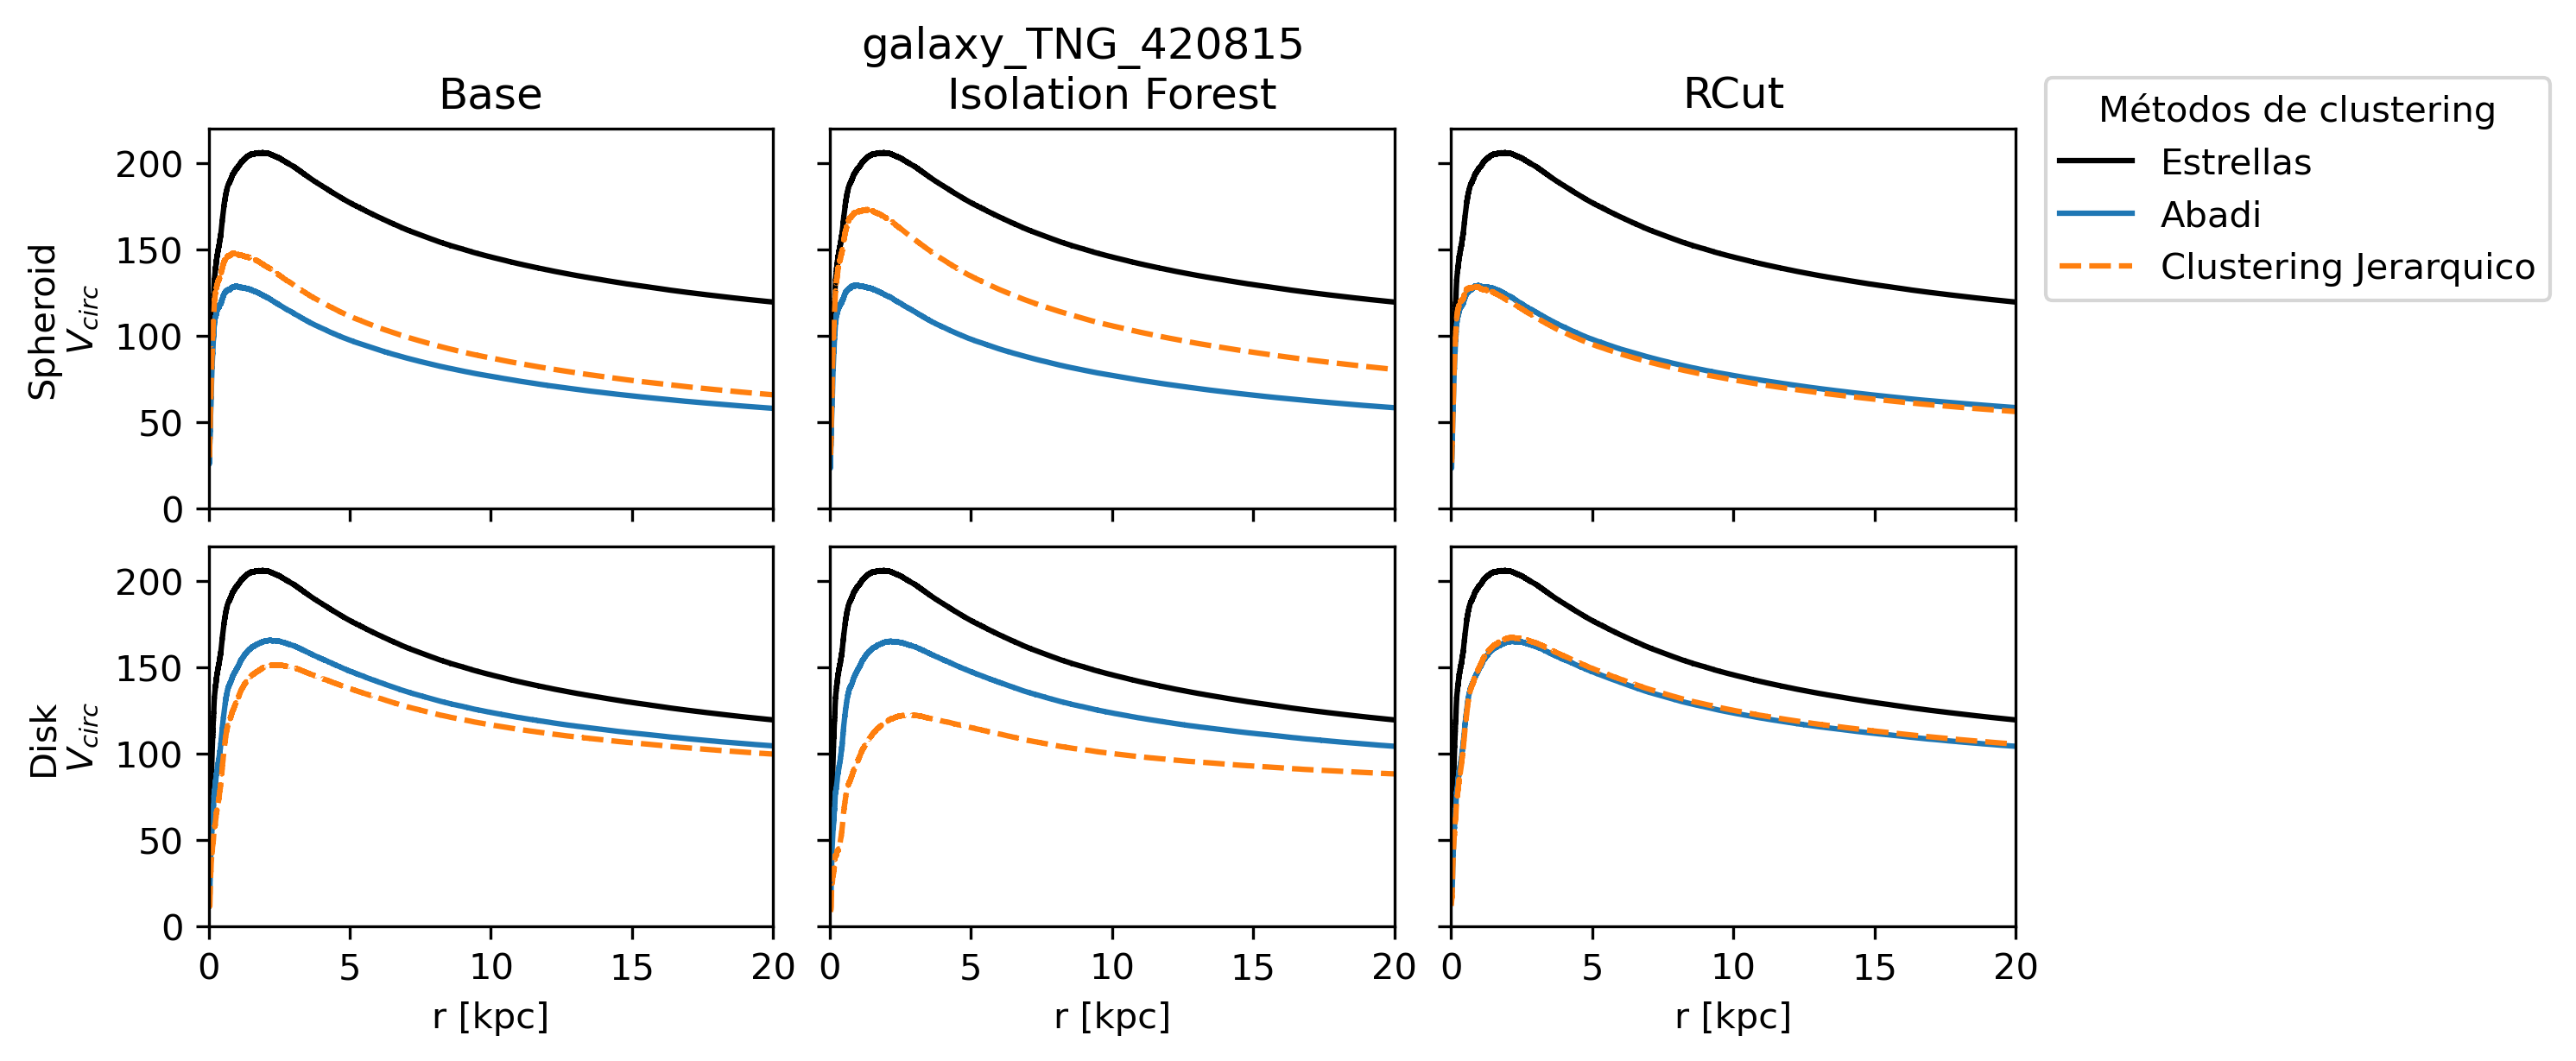
\includegraphics[width=11cm]{clustering jerarquico/figures/galaxy_TNG_420815 - Abadi - circ_velocity.png}
    \caption{Curva de rotación sobre los resultados obtenidos con Abadi y \gls{HC} sobre la galaxia \textit{galaxy\_TNG\_420815}, utilizando diferentes métodos de eliminación de outliers.}
    \label{fig:2componentesRotationCurve}
\end{figure}

\begin{table}[h!]
\centering
\begin{tabular}{l|l|c|c|c}
\cline{3-4}
\multicolumn{2}{c|}{}&Spheroid&Disk&\multicolumn{1}{c}{Total}\\
\cline{2-4}
& Abadi & $20322$ & $91202$ & $111524$\\
\cline{2-4}
& Ward & $26065$ & $85459$ & $111524$\\
\cline{2-4}
\end{tabular}
\caption{
    Comparación partículas estelares etiquetadas en cada componente por Abadi y \gls{HC} para la galaxia \textit{galaxy\_TNG\_420815}.
}
\label{table:2componentesCJ}
\end{table}


Tomando como \gls{GT} a Abadi, podemos ver que los valores obtenidos en las métricas de precision y recall (Fig~\ref{fig:2componentesAbadiPrecision}, y Fig~\ref{fig:2componentesAbadiRecall} columna 1) estan por arriba de $0.5$ y son bastante altos.

\begin{figure}
    \centering
    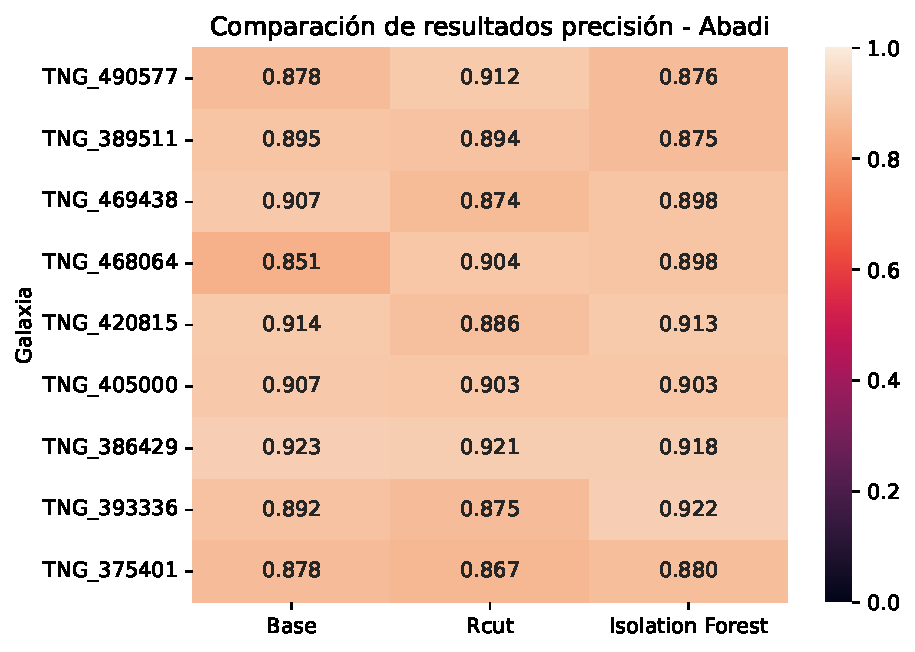
\includegraphics[width=12cm]{clustering jerarquico/figures/precision - abadi.pdf}
    \caption{Comparación de precisión sobre los resultados obtenidos entre Abadi y \gls{HC} con Ward.}
    \label{fig:2componentesAbadiPrecision}
\end{figure}

\begin{figure}
    \centering
    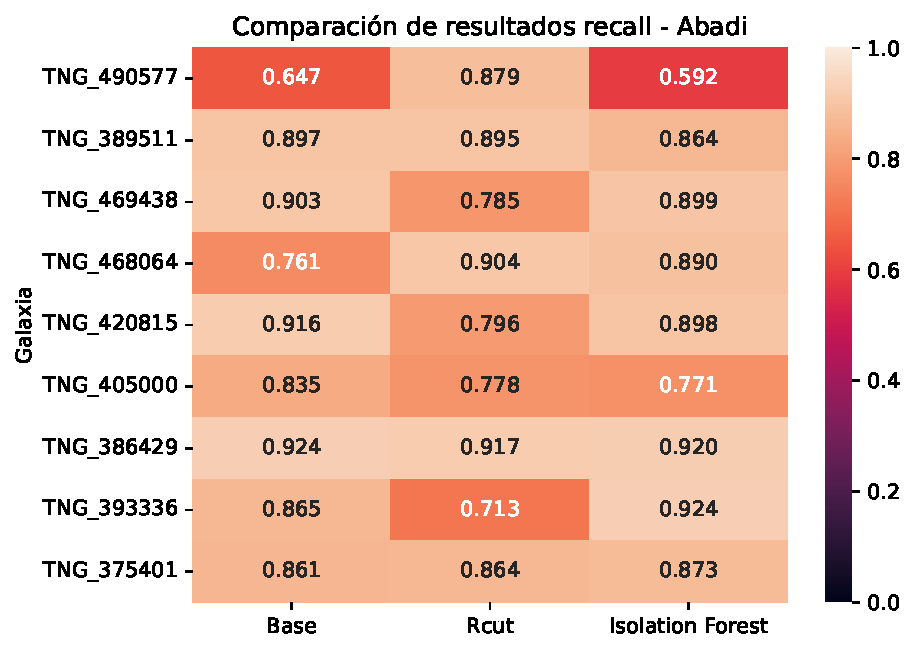
\includegraphics[width=12cm]{clustering jerarquico/figures/recall - abadi.pdf}
    \caption{Comparación de recall sobre los resultados obtenidos entre Abadi y \gls{HC} con Ward.}
    \label{fig:2componentesAbadiRecall}
\end{figure}

Si lo evaluamos con las métricas internas, podemos ver que Ward no presenta valores muy distintos a Abadi en la tabla de Silhouette (Fig~\ref{fig:2componentesAbadiSilhouette}), pero según Davis-Bouldin (primera y cuarta columna de la Fig~\ref{fig:2componentesAbadiDavisBouldin}) los clusters resultantes de Abadi son mucho más separados y con menos variación interna.

\begin{figure}
    \centering
    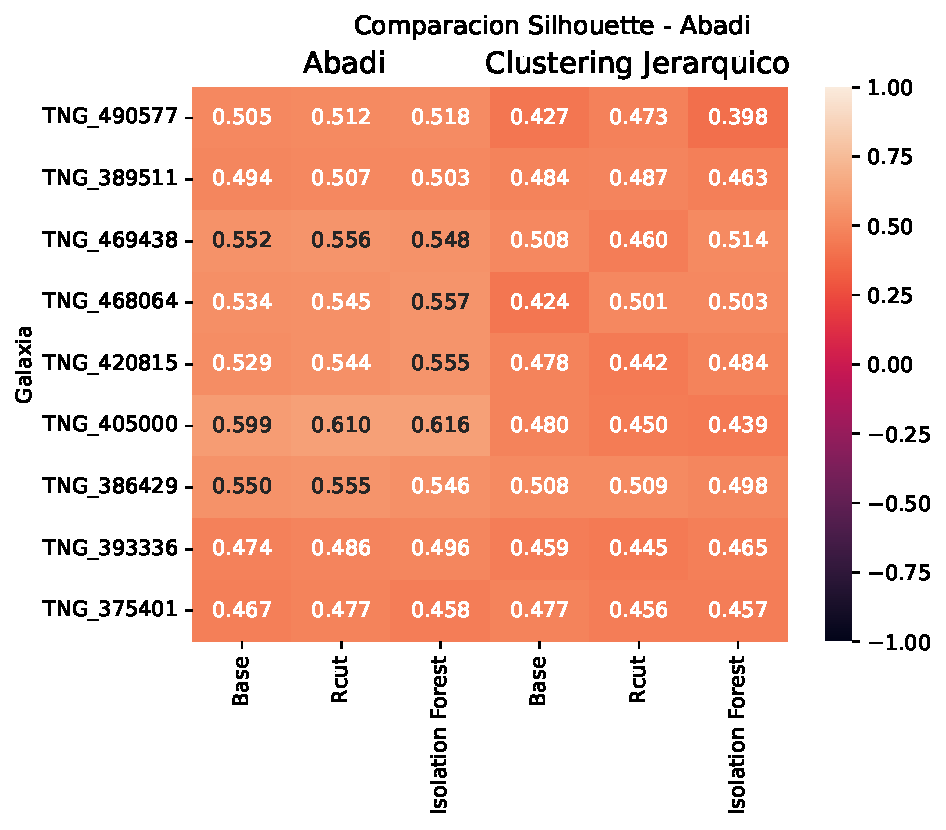
\includegraphics[width=12cm]{clustering jerarquico/figures/silhouette - abadi.pdf}
    \caption{Comparación de métrica Silhouette sobre los resultados obtenidos entre Abadi y \gls{HC} con Ward.}
    \label{fig:2componentesAbadiSilhouette}
\end{figure}

\begin{figure}
    \centering
    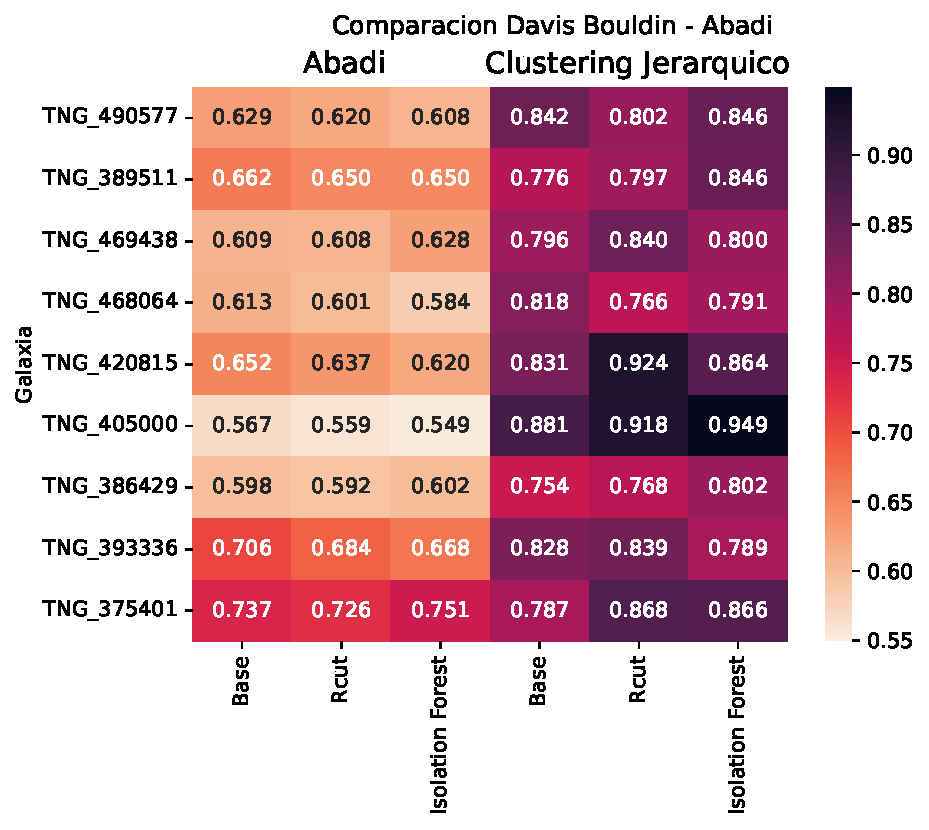
\includegraphics[width=12cm]{clustering jerarquico/figures/davis bouldin - abadi.pdf}
    \caption{Comparación de métrica Davies Bouldin sobre los resultados obtenidos entre Abadi y \gls{HC} con Ward.}
    \label{fig:2componentesAbadiDavisBouldin}
\end{figure}

Los resultados mostrados hasta el momento parecen converger a los obtenidos por el algoritmo de Abadi, dado que \gls{HC} logró encontrar una estructura similar a este último. Aunque Abadi tenga bases físicas, las cuales son más estables que un análisis meramente estadístico como el que realiza Ward, los artefactos que pueden observarse en los resultados obtenidos con \gls{HC} nos muestran que hay una tendencia a converger a los obtenidos con Abadi, reforzando así las bases ya establecidas por éste en el campo de investigación actual.

Dicho esto, los resultados obtenidos con \gls{HC} distan de ser tan buenos como los obtenidos por Abadi. \gls{HC} parece priorizar las partículas que están rotando a la hora de clasificar el disco, ya que éstas están más separadas del esferoide.

\vspace{15mm}

\subsection{Eliminación de outliers}

Como se mencionó brevemente en el capítulo anterior, el método de \gls{RCUT} se basa en eliminar las estrellas cuya distancia desde el centro de la galaxia supera cierto valor.

En la sección anterior, la aplicación de \gls{HC} sin trata de outliers sobre la galaxia 420815 parecía sobrestimar el esferoide. Podemos ver en la Fig~\ref{fig:2componentesRotationCurve} y la Fig~\ref{fig:2componentesCJRCutHistCirc} cómo, al aplicar \gls{RCUT}, las componentes encontradas parecen acercarse más a lo encontrado por Abadi (sobrestimando levemente el disco en el proceso). Interpretamos que la causa de dicho suceso fue que, dado que \gls{RCUT} remueve partículas estelares exteriores, y que el disco es la componente más externa de la galaxia, ésta será la componente que en mayor medida se verá afectada. Además, como es la componente con mayores valores de $eps$ (como la Fig~\ref{fig:2componentesCJRCutHistCirc} lo muestra en comparación a la Fig~\ref{fig:2componentesCJ}), el pico de densidad de ésta disminuirá, aumentando así la varianza sobre la componente Disco.

\begin{figure}
    \centering
    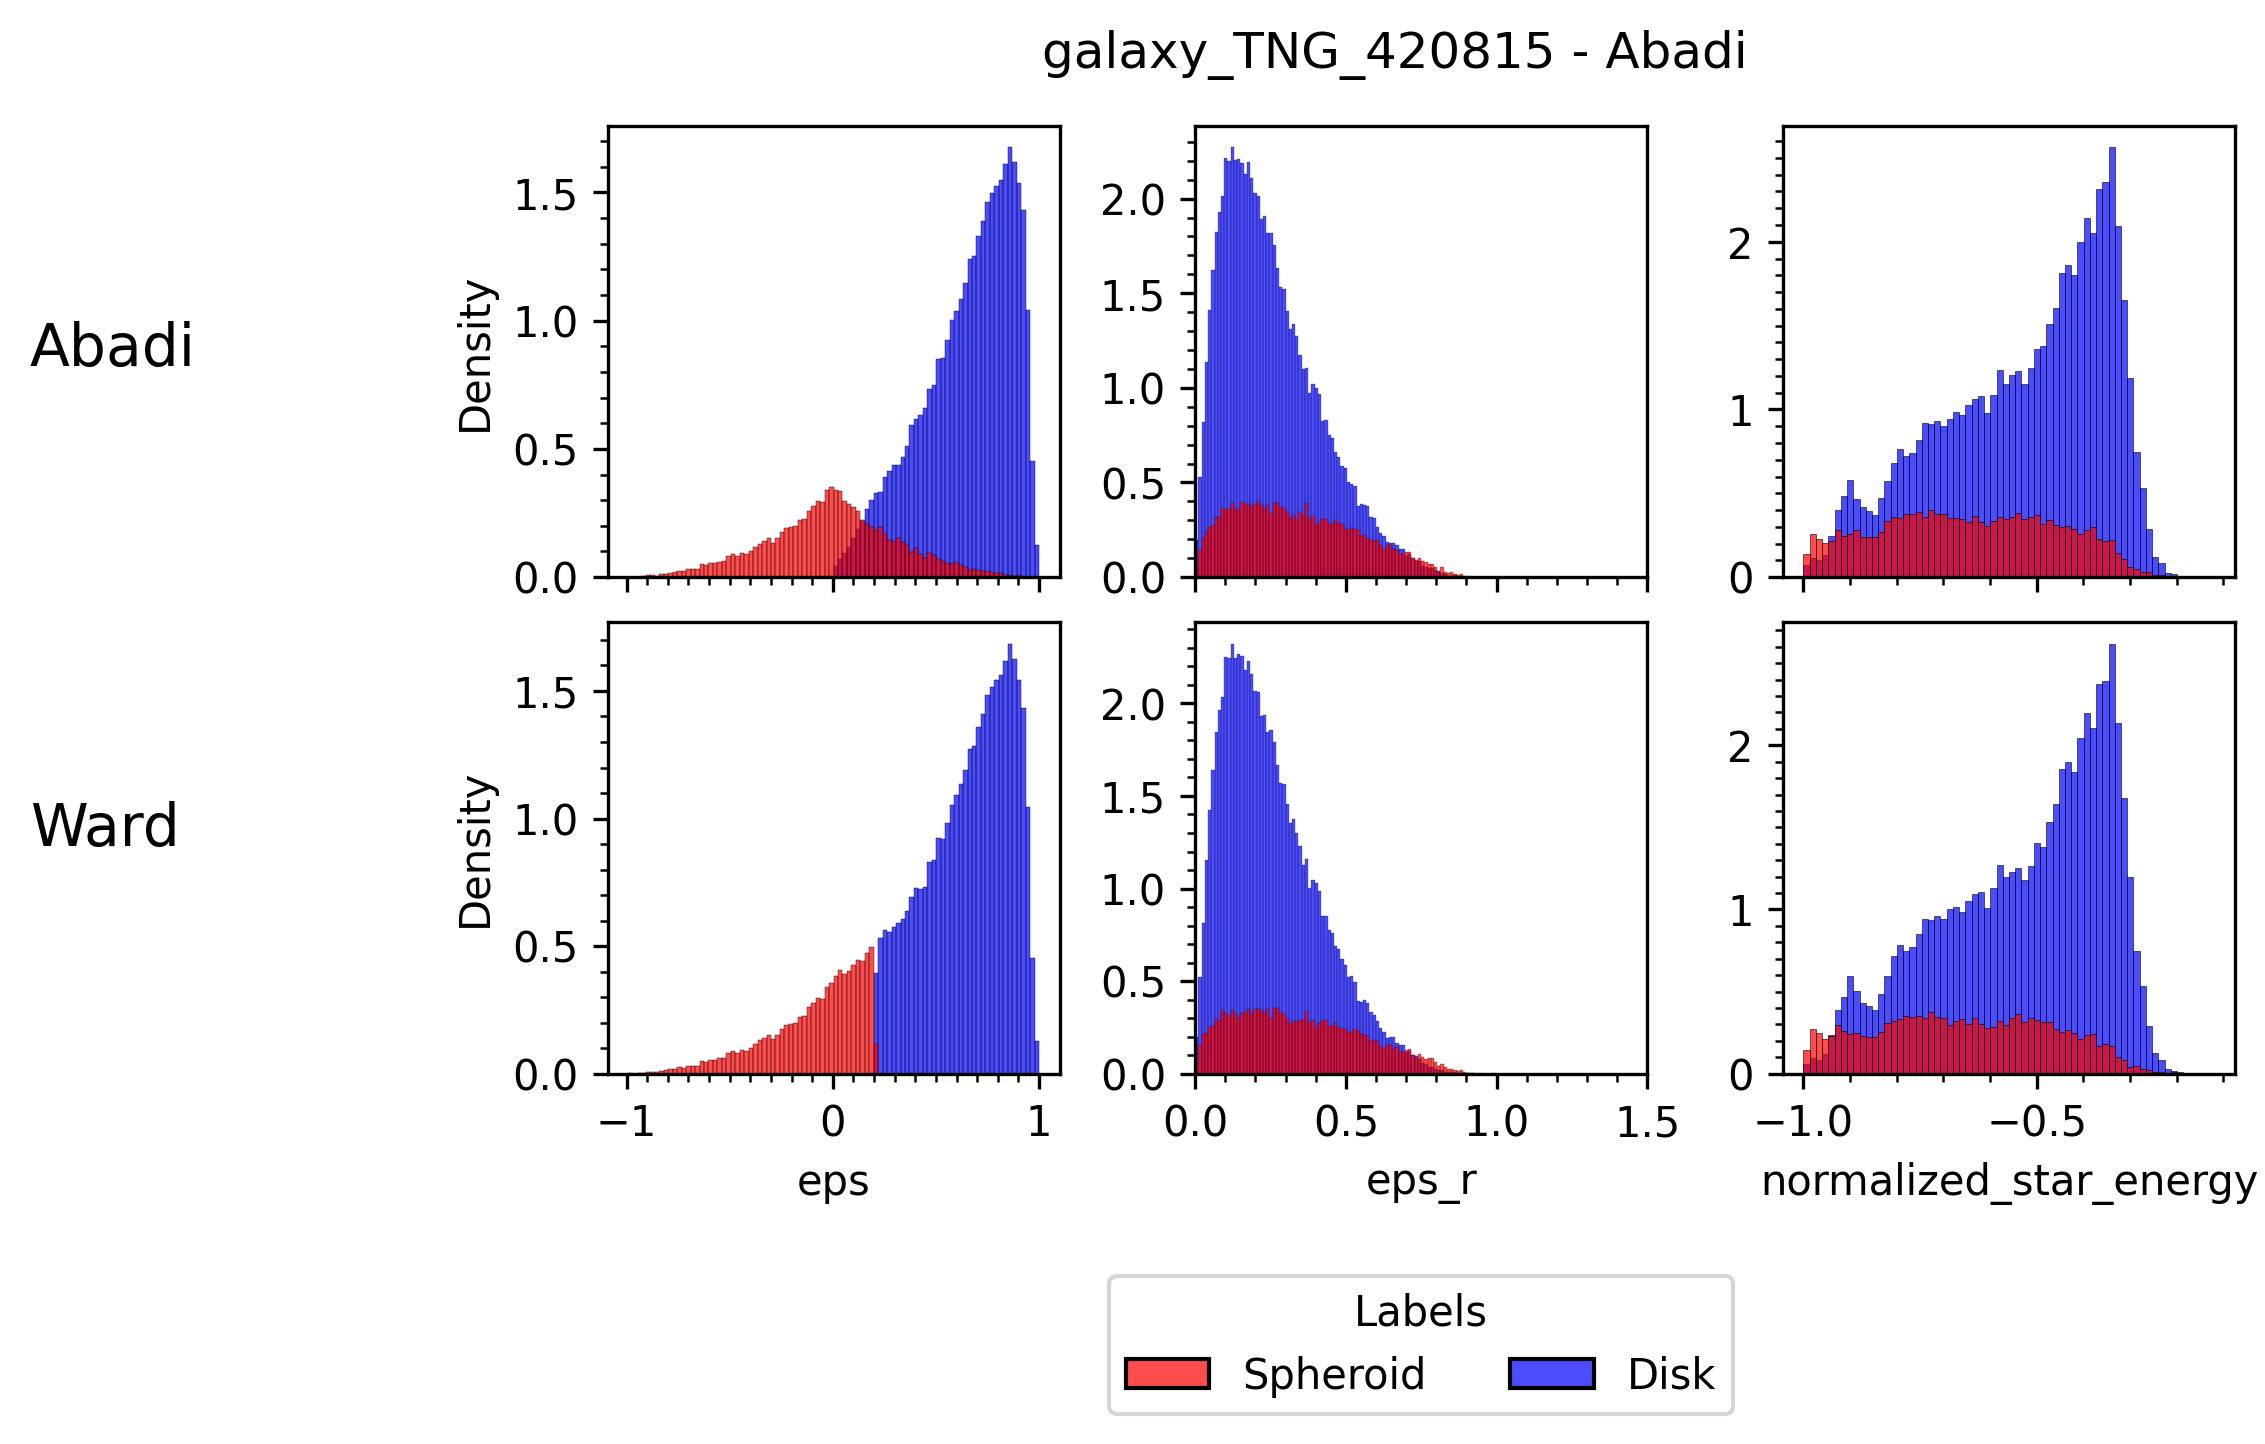
\includegraphics[width=11cm]{clustering jerarquico/figures/galaxy_TNG_420815 - abadi - rcut - circ histogram.png}
    \caption{Histograma comparando los resultados obtenidos con Abadi contra los obtenidos con \gls{HC} y linkage Ward, realizando eliminación de outliers con \gls{RCUT} sobre la galaxia \textit{galaxy\_TNG\_420815} en el espacio circular.}
    \label{fig:2componentesCJRCutHistCirc}
\end{figure}

Dado que en la Fig~\ref{fig:2componentesCJvsRCutvsIF_1} se puede observar que al eliminar outliers con \gls{RCUT} el pico de densidad de $eps$ desciende y la línea de corte en Ward se mueve hacia la derecha, es factible interpretar que dicho resultado proviene de la heurística de \gls{HC} de disminuir la varianza en sus componentes, y como la reducción del pico de densidad del Disco aumentó la varianza de éste, para compensar el mayor nivel de varianza del Disco, \gls{HC} mueve la línea de corte hacia la derecha.

\begin{figure}
    \centering
    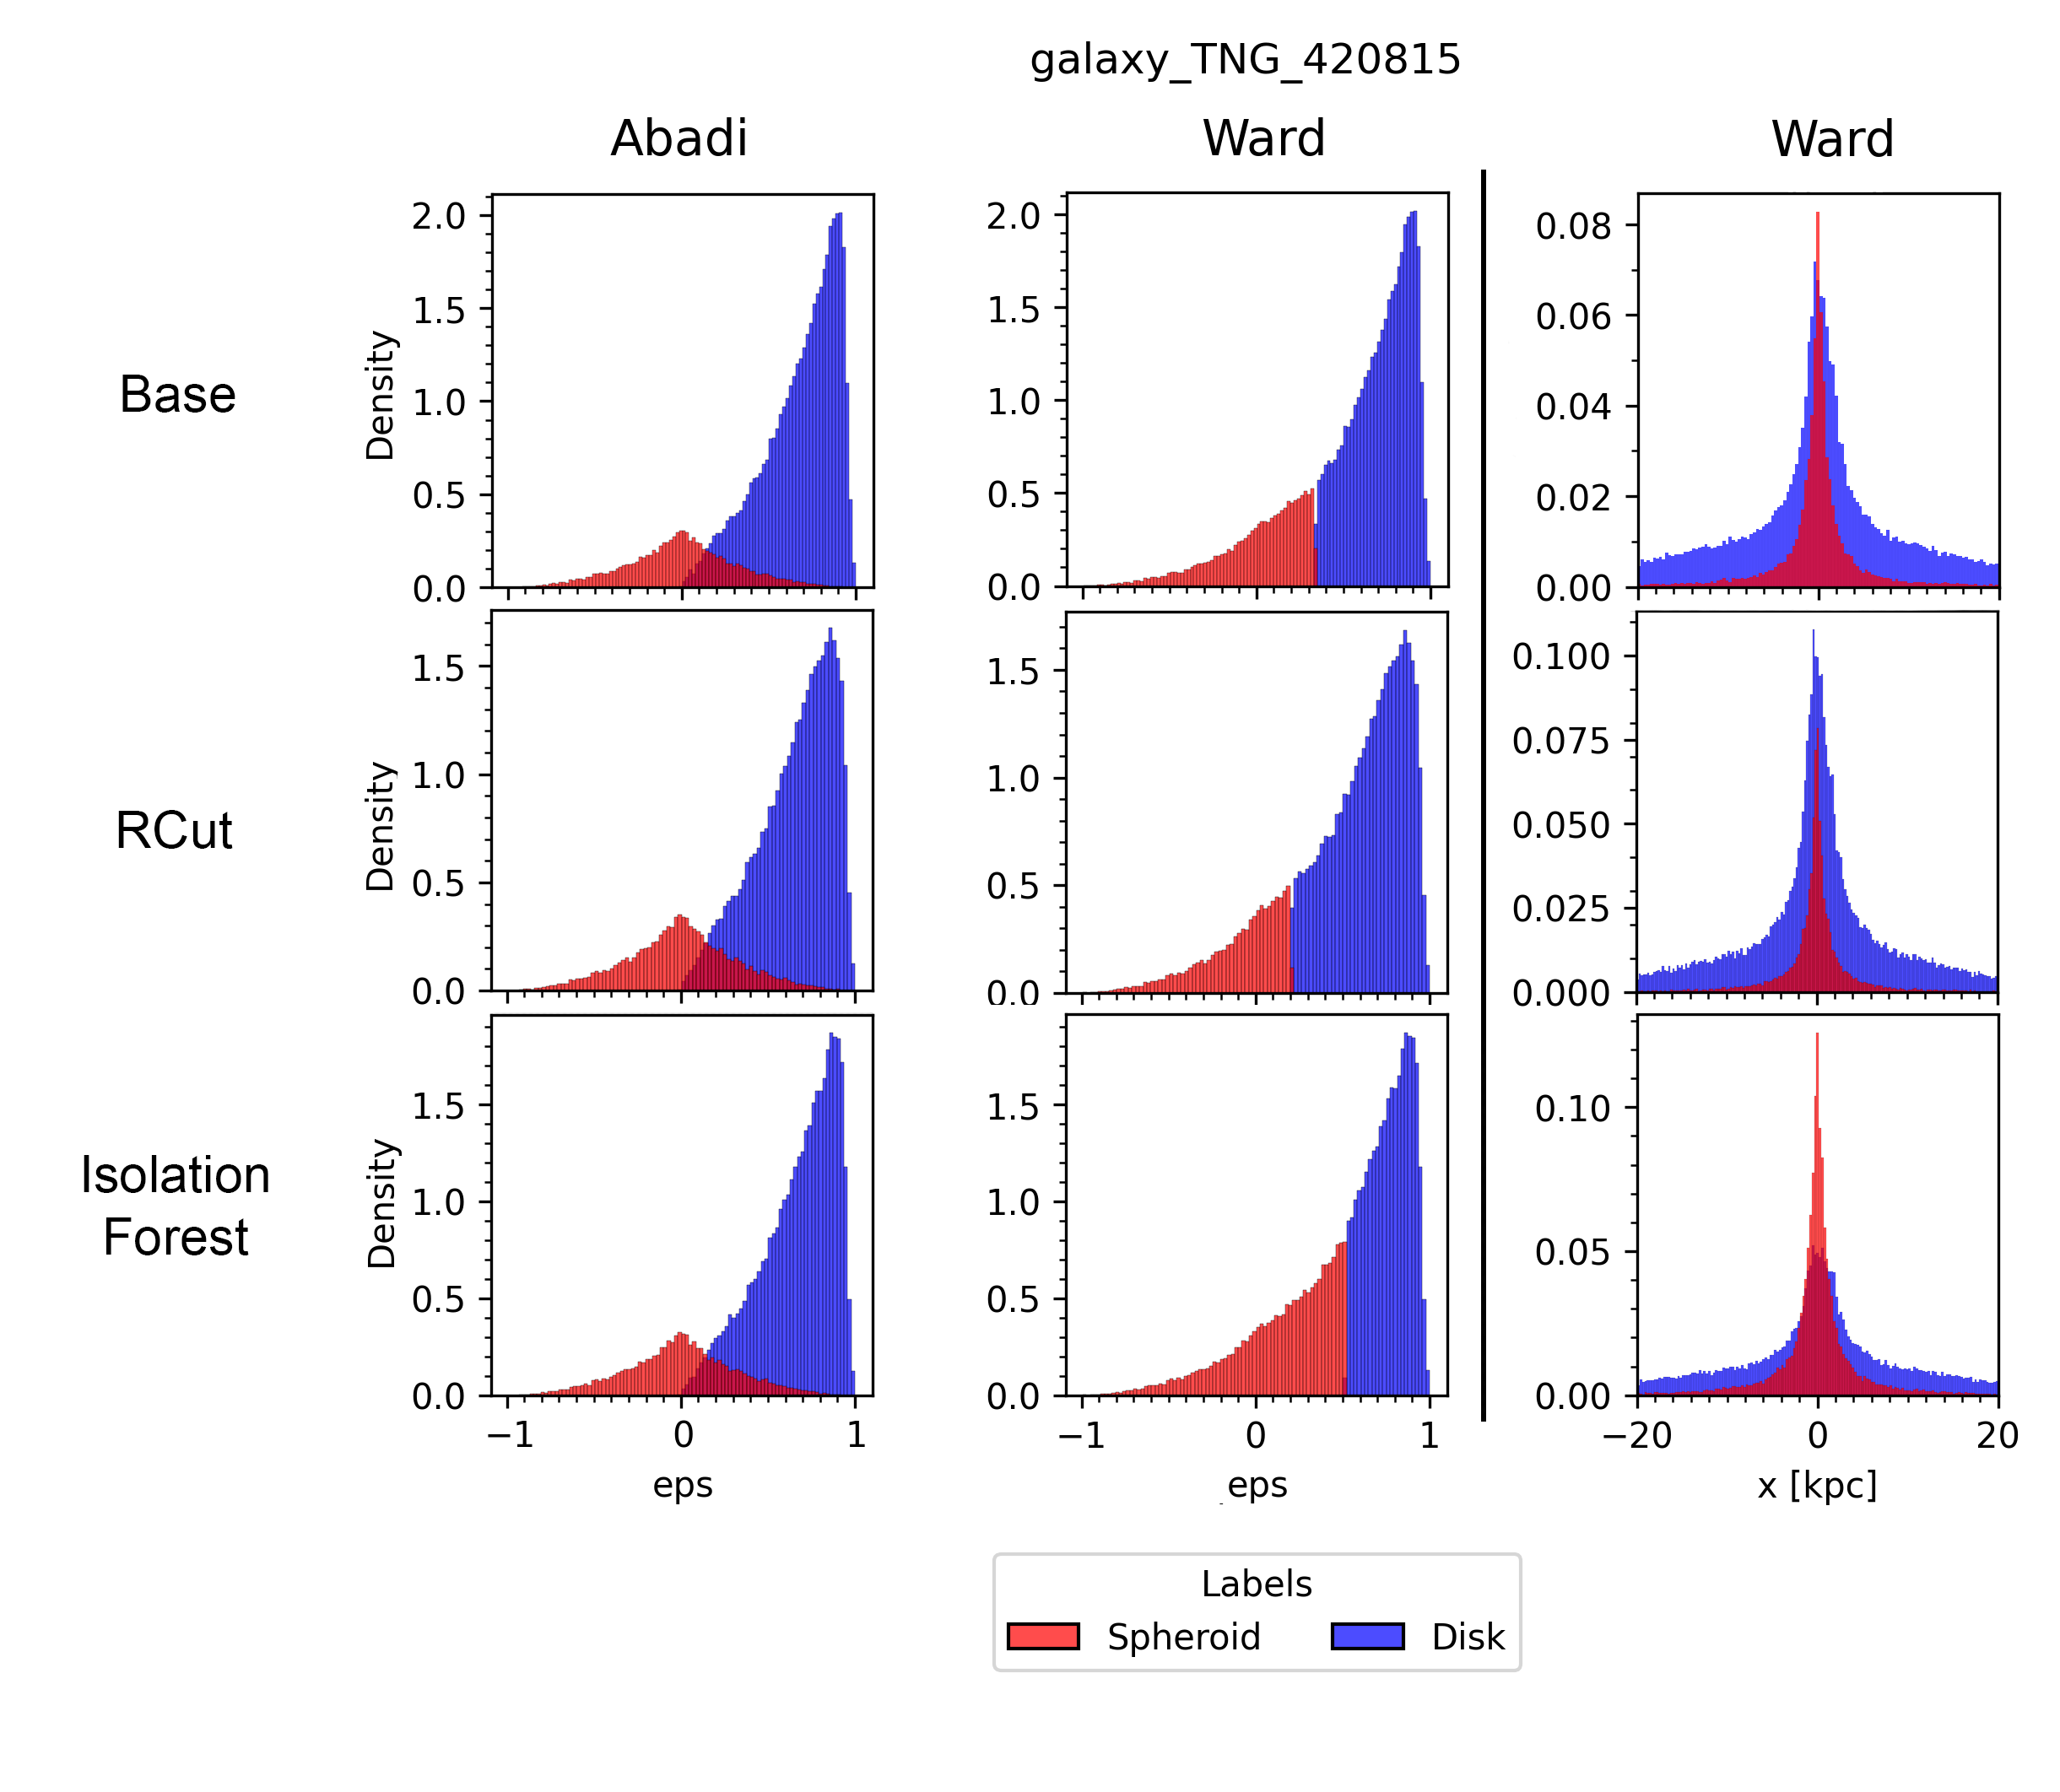
\includegraphics[width=11cm]{clustering jerarquico/figures/galaxy_TNG_420815 - abadi - base vs rcut vs isolation forest.png}
    \caption{Comparación de histogramas en espacio circular y real entre Abadi y \gls{HC} sin tratamiento de outliers, luego aplicando \gls{RCUT}, y luego aplicando \gls{IF} sobre la galaxia \textit{galaxy\_TNG\_420815}.}
    \label{fig:2componentesCJvsRCutvsIF_1}
\end{figure}

Sin embargo, los resultados mostrados en la Fig~\ref{fig:2componentesCJvsRCutvsIF_2} contradicen dicha hipótesis al mover la línea de corte hacia la izquierda al disminuir el pico de densidad de $eps$ cuando eliminamos outliers con \gls{RCUT} en Ward.

\begin{figure}
    \centering
    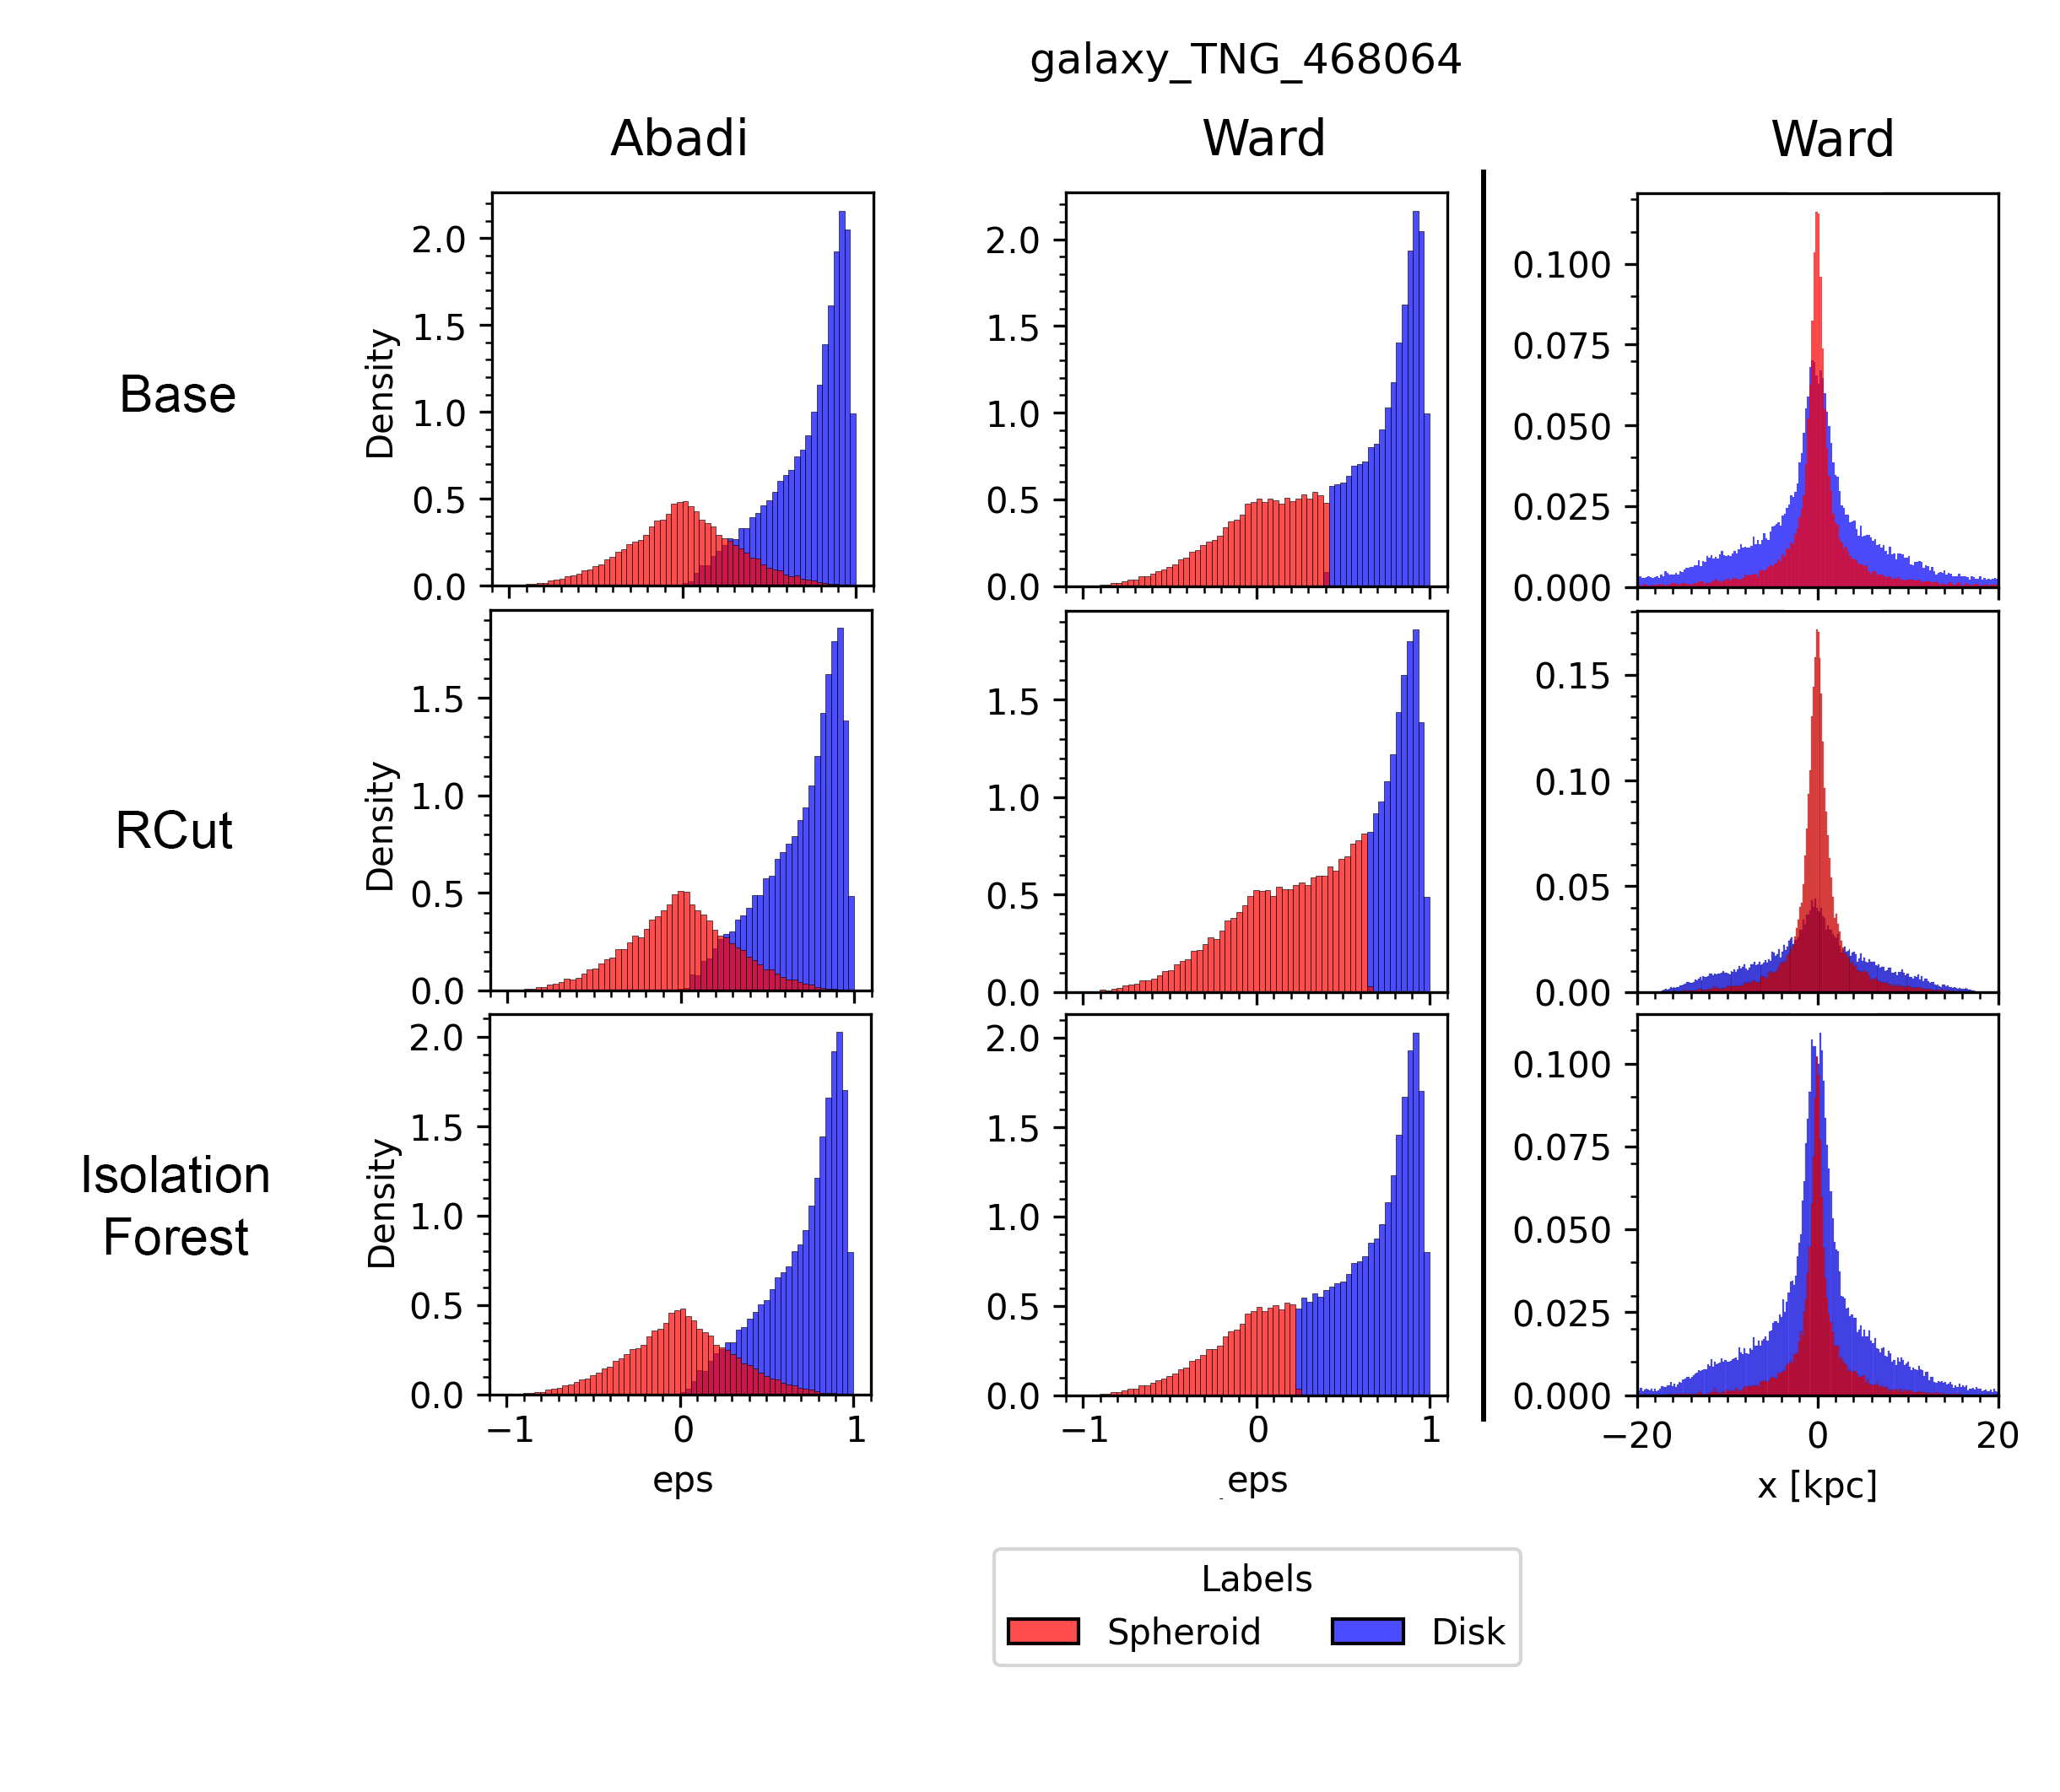
\includegraphics[width=11cm]{clustering jerarquico/figures/galaxy_TNG_468064 - abadi - base vs rcut vs isolation forest.png}
    \caption{Comparación de histogramas en espacio circular y real entre Abadi y \gls{HC} sin tratamiento de outliers, luego aplicando \gls{RCUT}, y luego aplicando \gls{IF} sobre la galaxia \textit{galaxy\_TNG\_468064}.}
    \label{fig:2componentesCJvsRCutvsIF_2}
\end{figure}

Al observar los histogramas de espacio circular y gráficas de velocidad del resto de las galaxias en el Apéndice~\ref{appendix}, no parece haber ninguna clara correlación entre las características de las galaxias y la forma en la que \gls{HC} encontrará sus componentes luego de remover outliers con \gls{RCUT}.

Por lo tanto, dado que remover outliers con \gls{RCUT} mueve el ``corte'' generado en $eps$ para Ward para la izquierda o derecha de forma arbitraria (independientemente de si se sobrestimó el disco o el esferoide en el análisis previo antes de remover outliers), no podemos concluir que \gls{RCUT} sea beneficioso para encontrar las componentes del Disco y el Esferoide en galaxias utilizando \gls{HC}.

En cuanto a \gls{IF}, dado que éste se basa en encontrar puntos fácilmente aislables en el espacio real, se eliminarán outliers en los tres ejes x, y, z. En este caso, dependiendo de la galaxia, no solo se eliminarán partículas del disco sino también del esferoide. Como las partículas del Disco son las más externas en el espacio real, dicha componente será la más afectada a la hora de remover outliers con este método, lo cual resulta en \gls{HC} moviendo la línea de ``corte'' en $eps$ entre el Esferoide y el Disco hacia la derecha para reducir la varianza de este último, la cual se vio incrementada en comparación con los resultados obtenidos antes de eliminar outliers. Puede apreciarse en la Fig~\ref{fig:2componentesCJvsRCutvsIF_1} un ejemplo de la tendencia de nuestro dataset a converger en este comportamiento, como así también en la Fig~\ref{fig:2componentesCJvsRCutvsIF_2} cómo remover outliers con \gls{IF} puede lograr el resultado opuesto en ciertas galaxias. Para más gráficas de circularidad y de velocidad sobre el resto de las galaxias referirse al Apéndice~\ref{appendix}.

Sin embargo, como sucedió con el método anterior, dado que dicha consecuencia solo nos es útil cuando aplicar Ward sin ningún tipo de tratamiento de outliers sobrestima el Disco (de forma tal que \gls{IF} pueda corregirlo), \gls{IF} no resulta de utilidad a la hora de buscar dos componentes con \gls{HC} ya que depende de cómo éstos varían respecto a los resultados con Abadi.

Dado lo que podemos observar al comparar los resultados con Abadi en la Fig~\ref{fig:2componentesAbadiPrecision}, con o sin remover outliers, se puede concluir que la aproximación de la densidad de cada cluster es bastante acertada. Mientras tanto, el heatmap de recall en la Fig~\ref{fig:2componentesAbadiRecall} nos muestra lo mucho que varió la certeza del Clustering Jerárquico entre varias galaxias.

Como nota final, podemos concluir que el \gls{HC} se comporta, como mucho, de forma similar a Abadi al buscar 2 clusters, pero como éste es más caro en memoria y computacionalmente (ya que calcula una matriz de distancia, por lo que estamos lidiando con magnitudes de $O(n^2)$ para ambos), el algoritmo de Abadi sigue siendo la mejor alternativa.

\section{Comparación con Auto Gaussian Mixture - $>$2 clusters}

Es necesario mencionar que, dado los malos resultados obtenidos por otros linkages al buscar dos componentes en la sección anterior, no sería de esperar que podamos obtener mejores resultados en esta sección, por lo cual no los revisaremos aquí.

Dado que ahora estamos buscando más de dos componentes, es natural pensar que dichas componentes surgirán de los clusters encontrados en la sección anterior. Es decir, si por ejemplo encontramos el Disco en una galaxia, es esperable que a la hora de buscar el Disco Fino y el Disco Grueso, las partículas estelares de ambos estén incluidos en la componente Disco original (o al menos una gran parte de ellas). Esto no es un problema para la componente utilizada como ejemplo, pero se vuelve un inconveniente a la hora de buscar el Halo y el Bulge dentro del Esferoide.

Dado que el Esferoide es una componente soportada por dispersión de velocidades, sus partículas estelares tiene una alta variación en $eps$ \citep{mo2010galaxy}. Como las componentes Halo y Bulge dependen del movimiento que predomina en el Esferoide, los valores de $eps$ de sus partículas estelares tendrán una alta variación. Y, por consecuente, ambas componentes se verán ``solapadas'' en $eps$, como bien puede observarse en la grafica de \gls{AGMM} en la Fig~\ref{fig:agmm_circ_hist_1}.

\begin{figure}
    \centering
    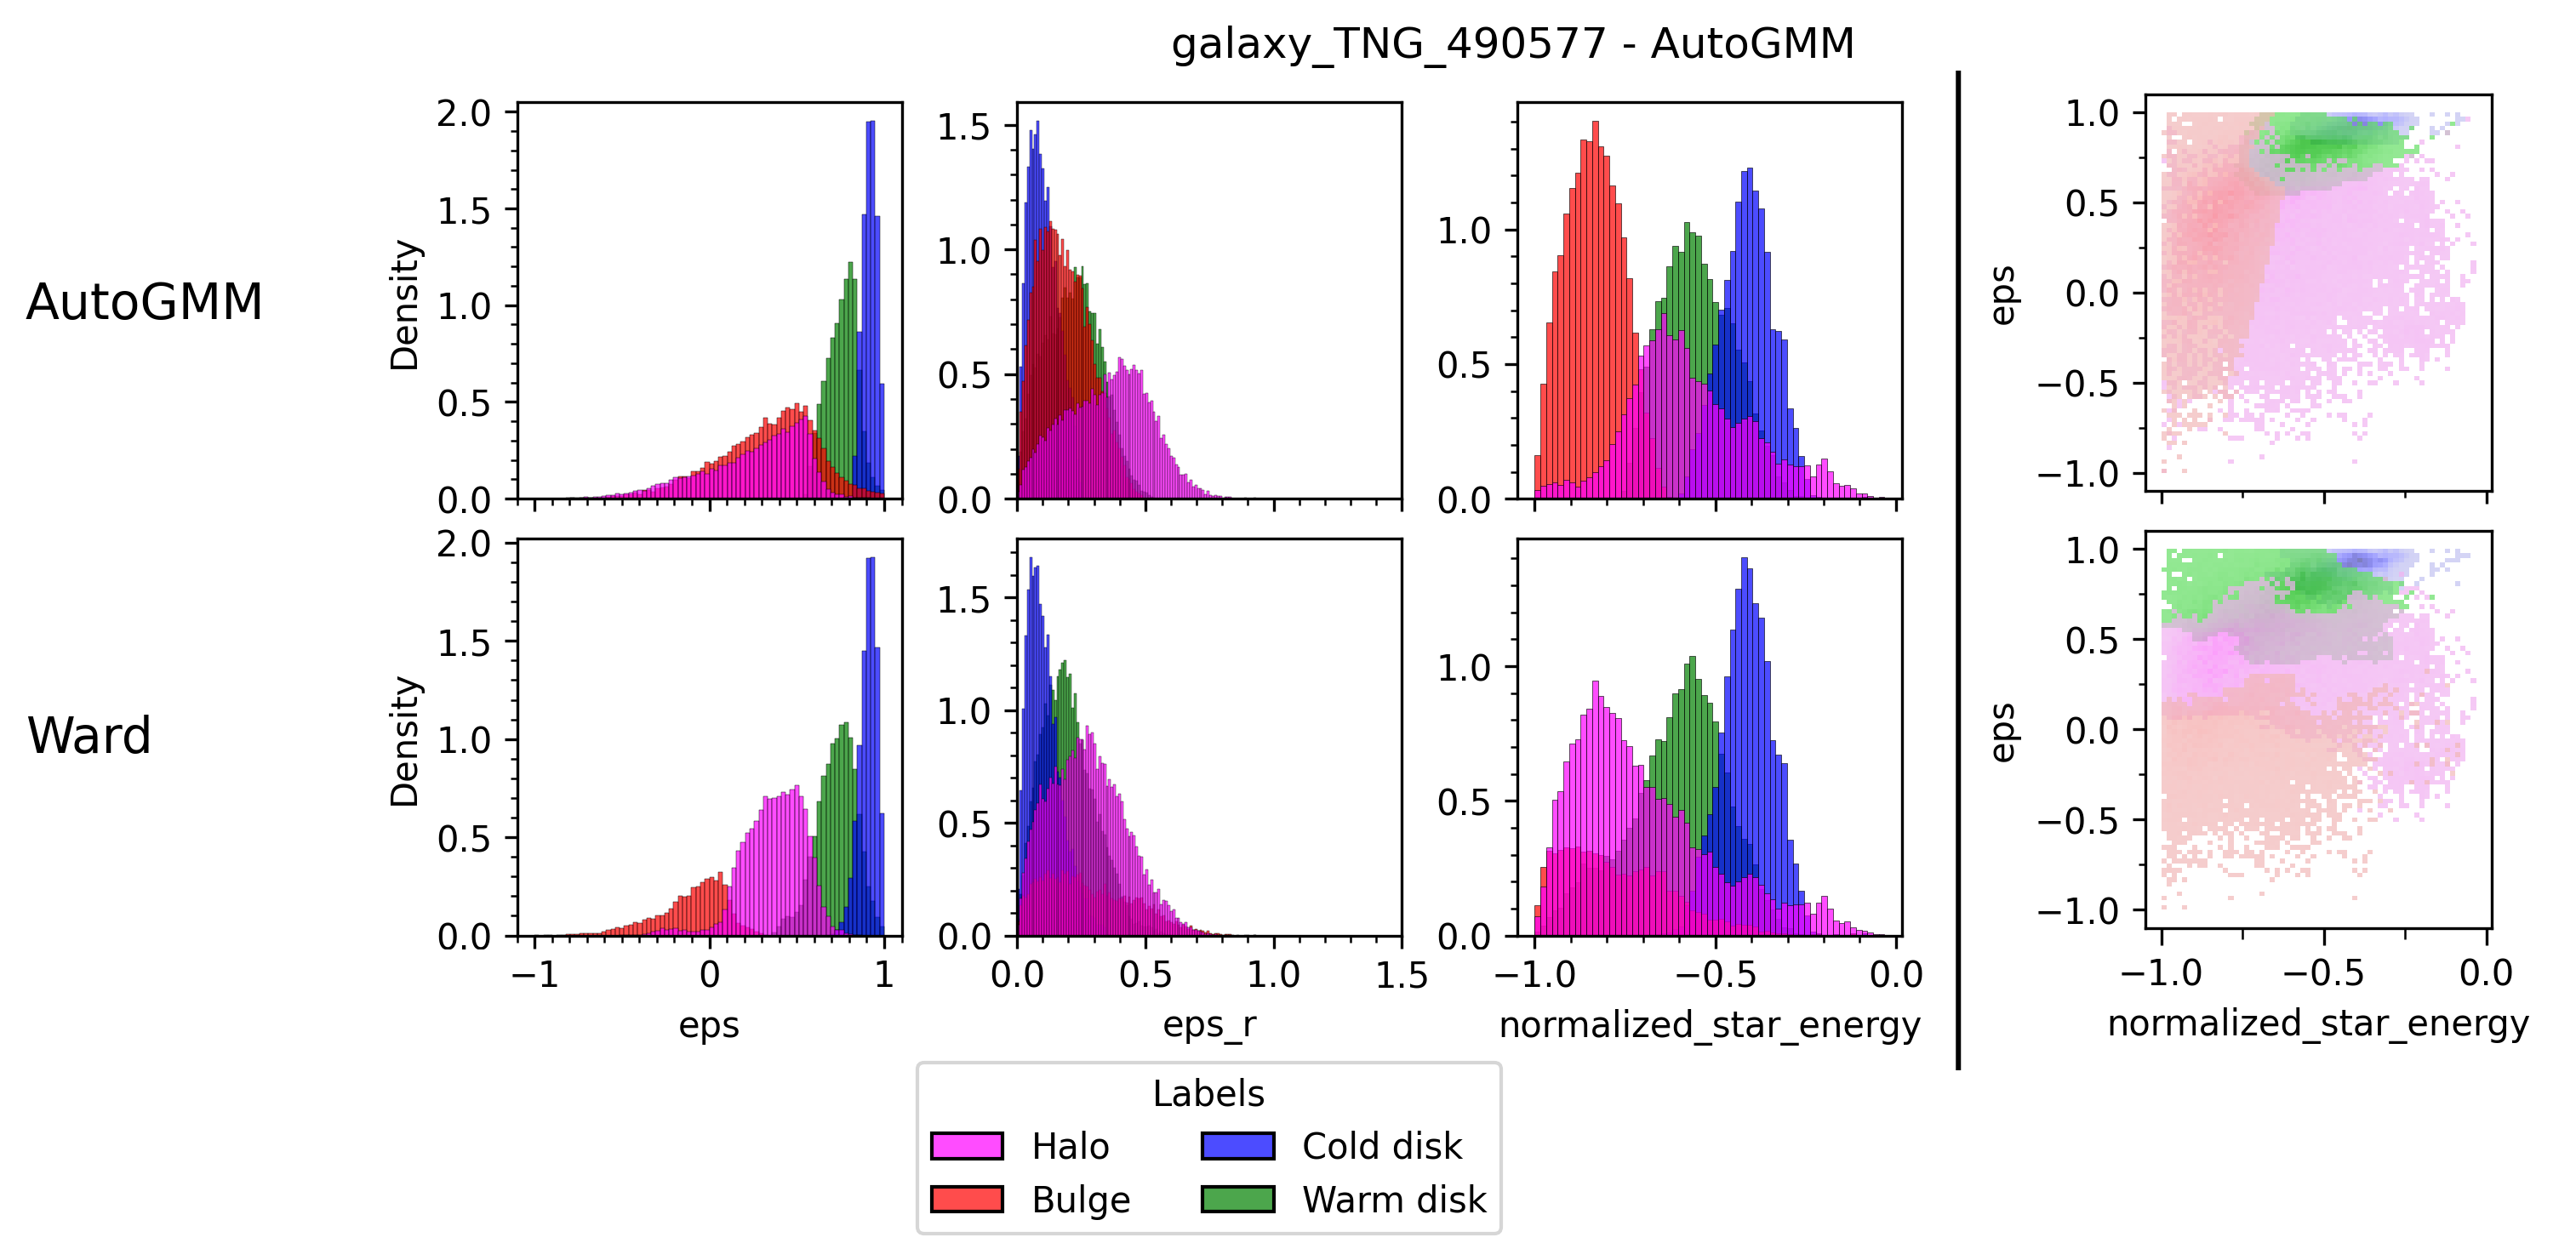
\includegraphics[width=.9\textwidth]{clustering jerarquico/figures/AGMM - galaxy_TNG_490577 - circ histogram.png}
    \caption{\label{fig:agmm_circ_hist_1} Histograma comparando los grupos obtenidos con \gls{HC} contra \gls{AGMM} sobre la galaxia \textit{galaxy\_TNG\_490577} en el espacio circular.}
\end{figure}

Como \gls{HC} busca minimizar la varianza de cada cluster, esto se traduce en buscar que los clusters estén lo más separados entre ellos, lo cual va en directa contraposición con la naturaleza de las componentes mencionadas al observar el histograma de $eps$, incluso si dicha heurística tiene sentido dentro del marco teórico del agrupamiento de datos.

Esta distinción entre lo que es más correcto a la hora de buscar clusters abstractos contra buscar componentes de una galaxia se vuelve aún más evidente si revisamos las métricas de Silhouette y Davies-Bouldin en la Fig~\ref{fig:NcomponentesAGMMSilhouette} y Fig~\ref{fig:NcomponentesAGMMDavisBouldin} respectivamente. Estas métricas son calculadas a partir del concepto ideal abstracto de cluster, el cual se basa en que éstos sean compactos, separados espacialmente entre ellos, y que exista ``continuidad'' en cada uno. Los resultados de estas métricas apuntan a que las componentes encontradas por Ward son más correctas que las encontradas por \gls{AGMM}, cuando esto no se corresponde en realidad con las estructuras de las galaxias.

\begin{figure}
    \centering
    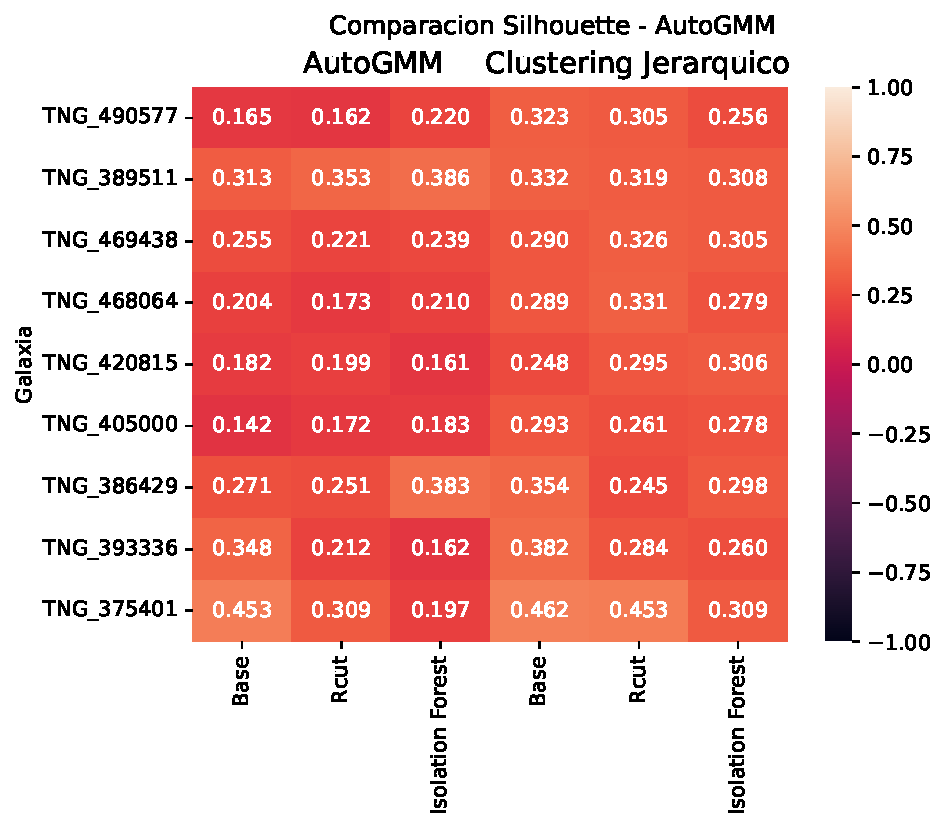
\includegraphics[width=12cm]{clustering jerarquico/figures/silhouette - agmm.pdf}
    \caption{Comparación de métrica Silhouette sobre los resultados obtenidos entre \gls{AGMM} y \gls{HC} con Ward.}
    \label{fig:NcomponentesAGMMSilhouette}
\end{figure}

\begin{figure}
    \centering
    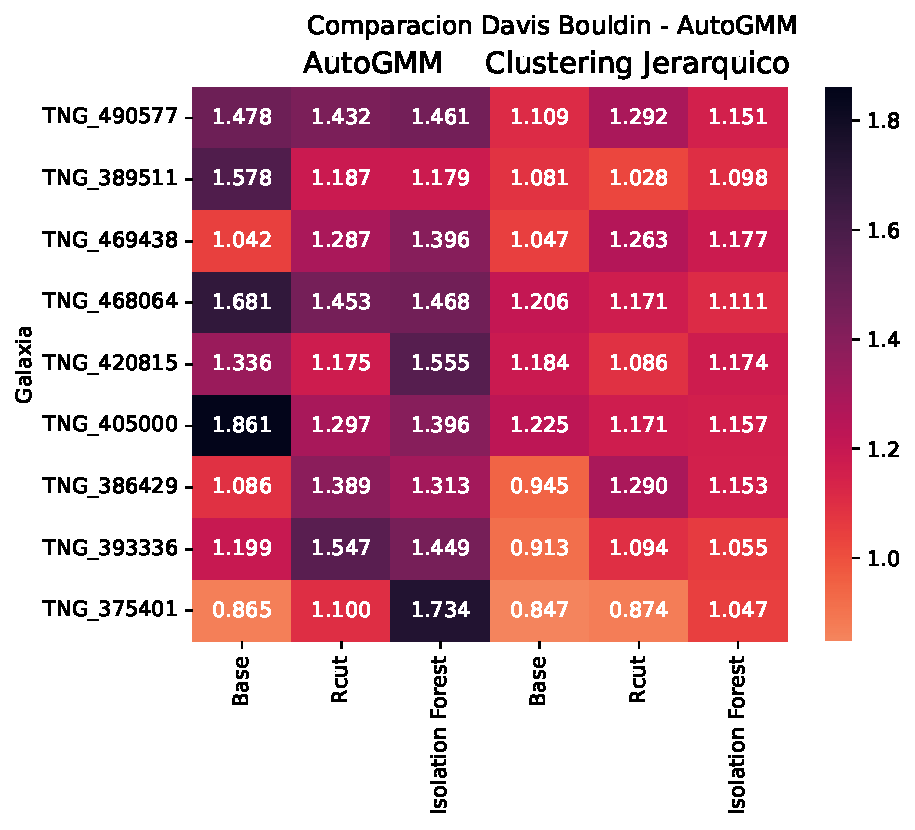
\includegraphics[width=12cm]{clustering jerarquico/figures/davis bouldin - agmm.pdf}
    \caption{Comparación de métrica Davies Bouldin sobre los resultados obtenidos entre \gls{AGMM} y \gls{HC} con Ward.}
    \label{fig:NcomponentesAGMMDavisBouldin}
\end{figure}

Esto conlleva a que $eps$ no sea una feature útil para Ward a la hora de diferenciar las dos componentes mencionadas. De las dos features restantes, $normalized\_star\_energy$ sería la más prometedora según el orden de relevancia en el área. La importancia de dicha feature se ve reforzada al observar las componentes identificadas por \gls{AGMM} en la Fig~\ref{fig:agmm_circ_hist_2}, en donde se puede ver una clara separación entre el Halo y el Bulge que podría resultar útil para \gls{HC}. Sin embargo, la existencia de más clusters con partículas estelares ``solapando'' a ambos el Halo y el Bulge en los mismos valores de $normalized\_star\_ernergy$ conlleva a que Ward se concentre en la clusterización que es posible derivar de $eps$. Esto resulta en un agrupamiento casi exclusivamente unidimensional y claramente erróneo, como se puede ver en el scatterplot de la Fig~\ref{fig:agmm_circ_hist_2}.

\begin{figure}
    \centering
    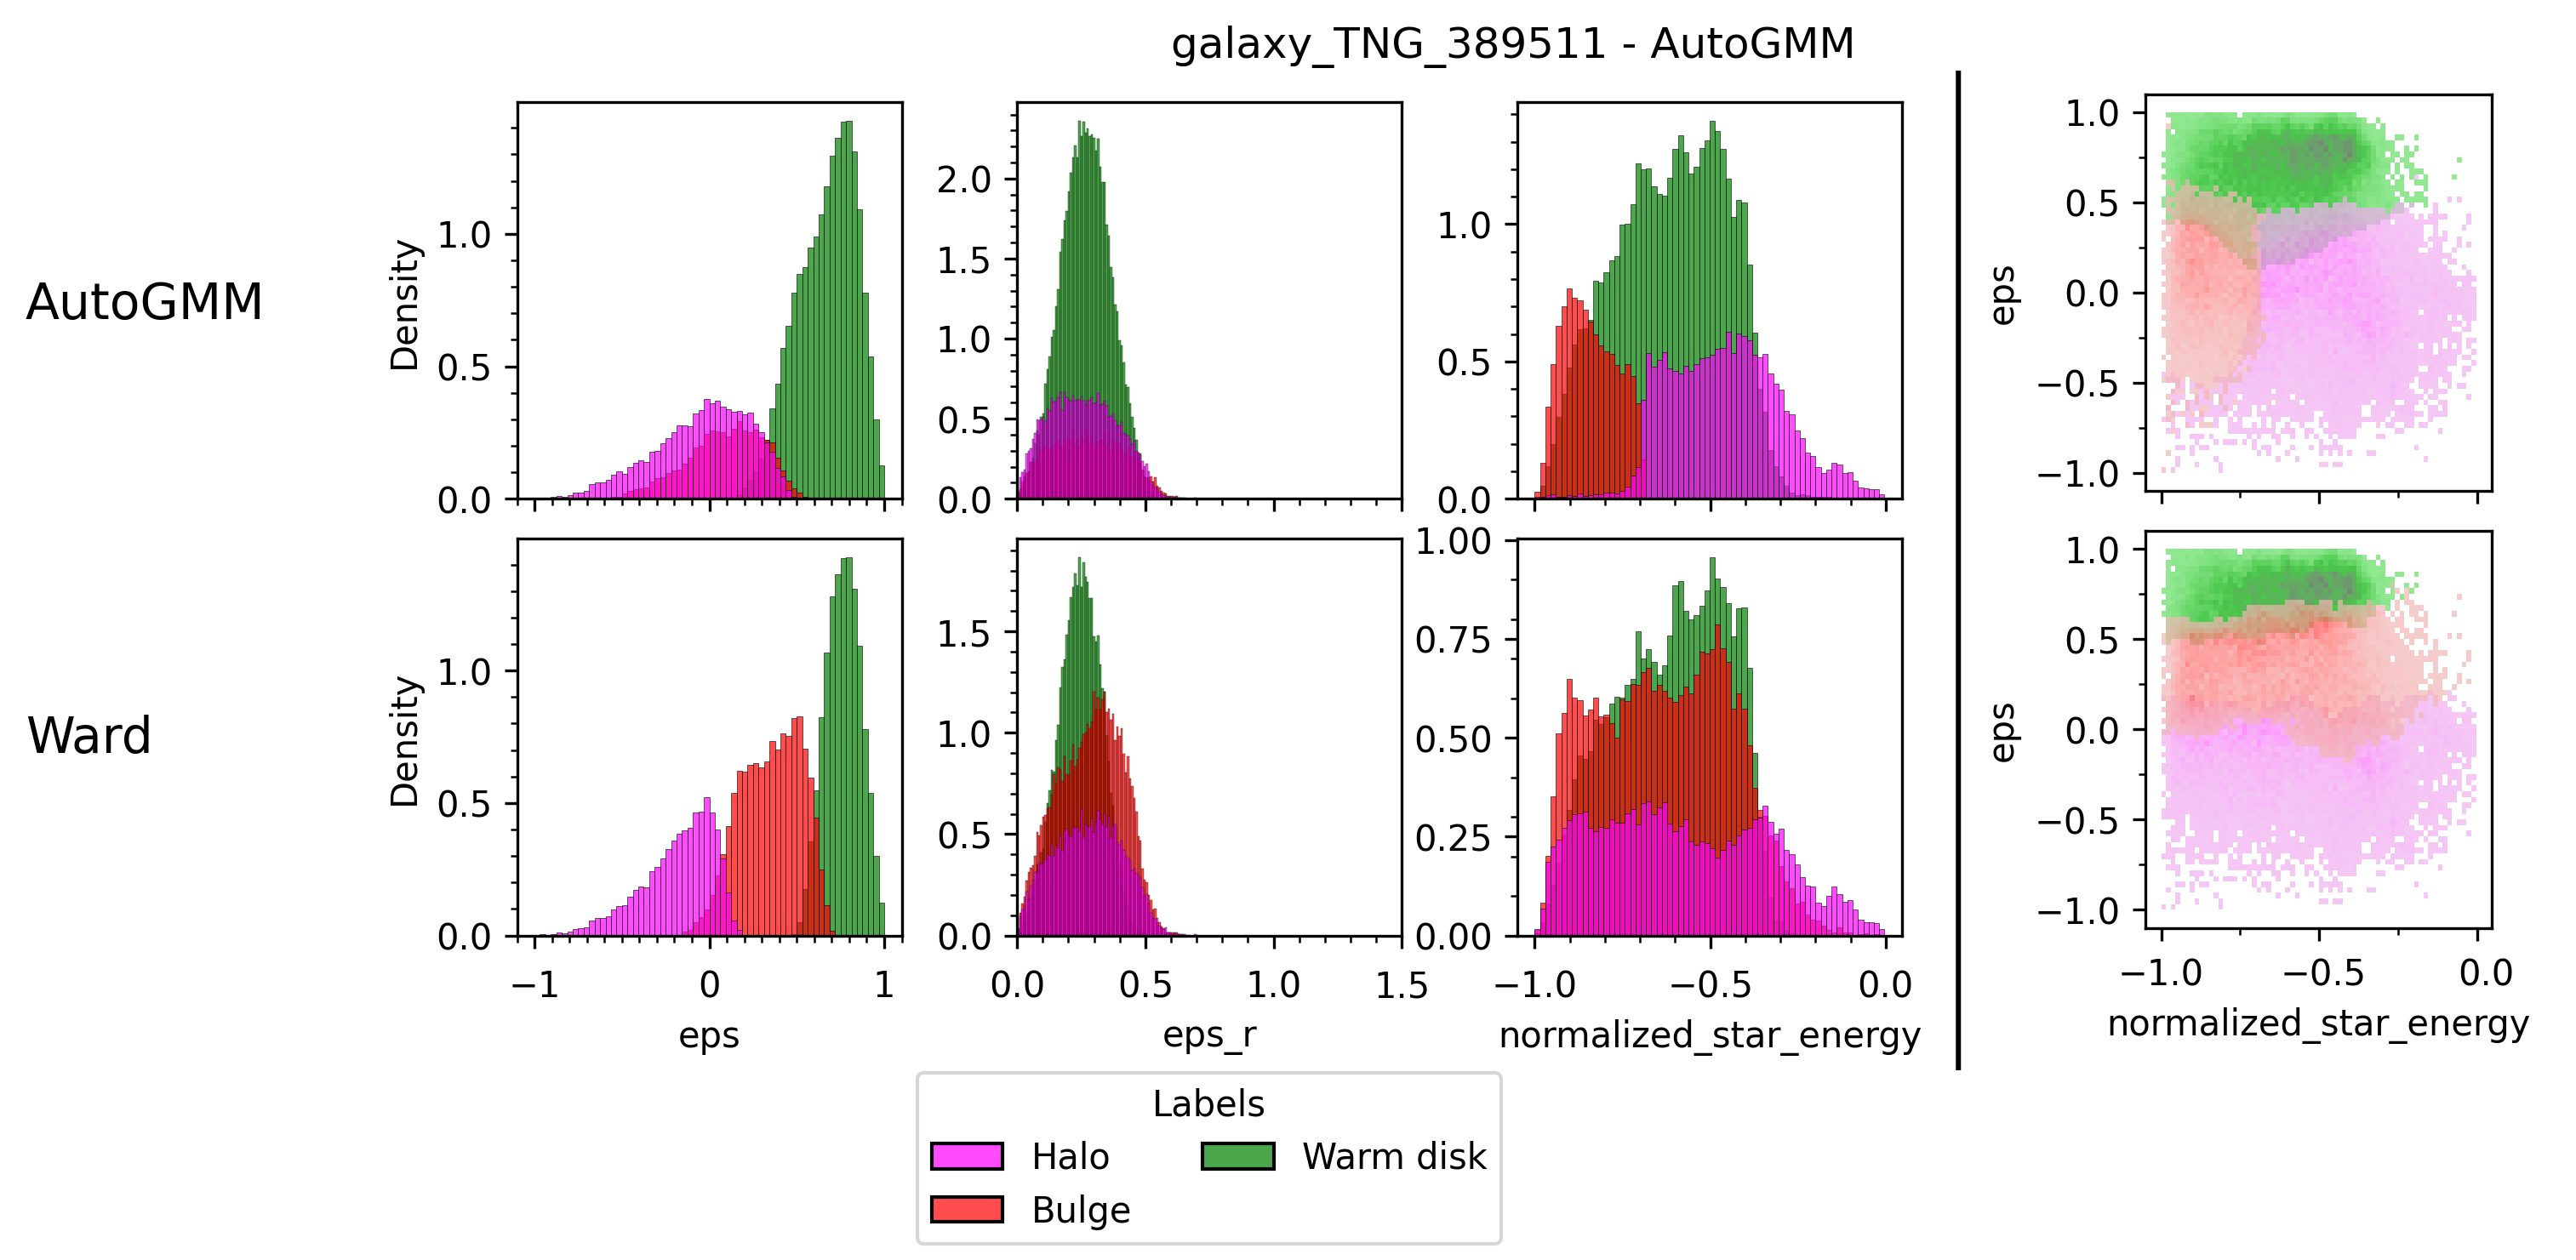
\includegraphics[width=.9\textwidth]{clustering jerarquico/figures/AGMM - galaxy_TNG_389511 - circ histogram}
    \caption{\label{fig:agmm_circ_hist_2} Histograma comparando los grupos obtenidos con \gls{HC} contra \gls{AGMM} sobre la galaxia \textit{galaxy\_TNG\_389511} en el espacio circular.}
\end{figure}

Diferente es, por ejemplo, si se busca el Disco Fino y el Disco Grueso. Como las componentes del Disco son soportadas por rotación, esto significa que predomina el movimiento ordenado \citep{mo2010galaxy}, y las dispersiones en $eps$ de ambos grupos son más acotadas en comparación a las componentes del esferoide (con el Disco Grueso en particular teniendo más varianza que el Disco Fino). Esto implica que \gls{HC} tenga una mayor facilidad a la hora de identificar dichas componentes, como bien puede observarse en la Fig~\ref{fig:agmm_circ_hist_1}.

Además, como el promedio de los valores de precisión obtenidos en las 9 galaxias de nuestro conjunto de prueba es de 0.65 (Fig~\ref{fig:NcomponentesAGMMPrecision}), mientras que el de recall es de 0.58 (Fig~\ref{fig:NcomponentesAGMMRecall}), podemos afirmar con un alto nivel de certeza que \gls{HC} no hace un buen trabajo al buscar más de dos componentes. Esto tiene sentido ya que las soluciones del método jerárquico con más clusters son particiones de las soluciones con menos clusters, por lo cual solo pueden aumentar el error al aumentar la cantidad de clusters a buscar.

\begin{figure}
    \centering
    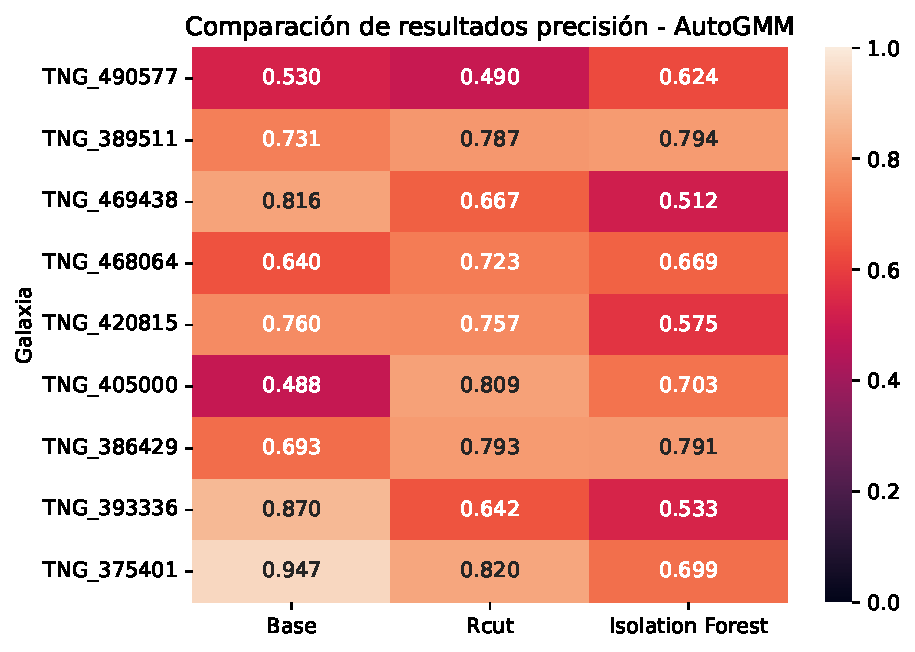
\includegraphics[width=12cm]{clustering jerarquico/figures/precision - agmm.pdf}
    \caption{Comparación de precisión sobre los resultados obtenidos entre \gls{AGMM} y \gls{HC} con Ward.}
    \label{fig:NcomponentesAGMMPrecision}
\end{figure}

\begin{figure}
    \centering
    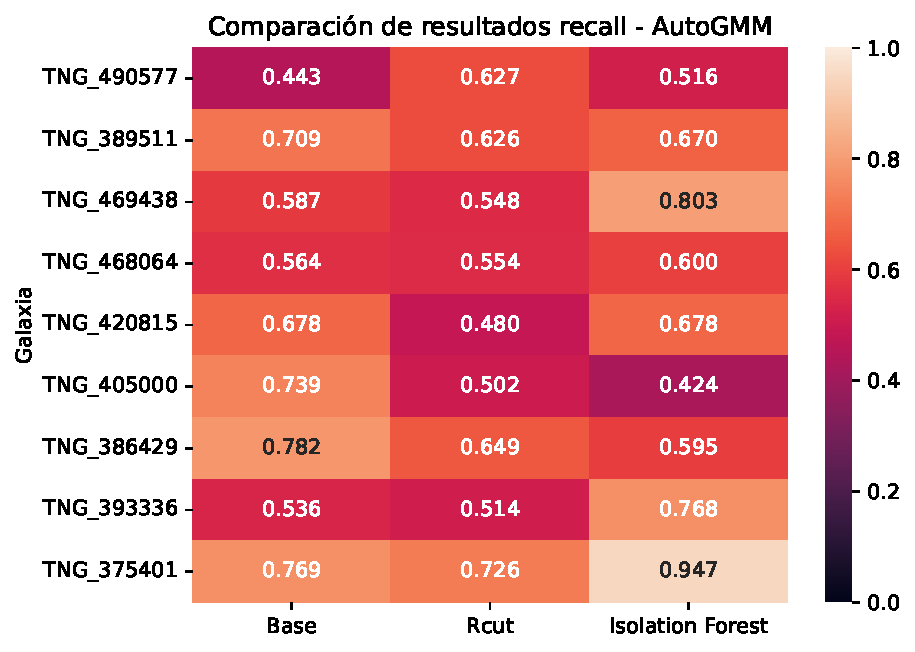
\includegraphics[width=12cm]{clustering jerarquico/figures/recall - agmm.pdf}
    \caption{Comparación de recall sobre los resultados obtenidos entre \gls{AGMM} y \gls{HC} con Ward.}
    \label{fig:NcomponentesAGMMRecall}
\end{figure}

Similar a como sucedió con Abadi, los resultados tienen una leve tendencia de converger a los obtenidos con \gls{AGMM}. Aun así, nuevamente, la clusterización obtenida con \gls{HC} dista de ser tan buena como la obtenida por \gls{AGMM}, por lo cual este último método sigue siendo preferible.

\subsection{Eliminación de outliers}

Es necesario remarcar que para asignar labels a los clusters encontrados por \gls{HC} (y los métodos de los siguientes capítulos) utilizamos una heurística que resuelve el “labels map”. Es decir, una función que asocia un cluster a un componente de la galaxia. En este caso nuestra asignación automática maximiza el promedio pesado de los valores de Recall de cada conjunto encontrado de entre todas sus posibles permutaciones. Por lo cual, aunque pareciera que en la Fig~\ref{fig:AGMM490577Complete} hemos etiquetado de forma errónea al Halo y el Bulge en \gls{IF}, el método detallado nos provee una base sólida para razonar sobre los resultados.

\begin{figure}
    \centering
    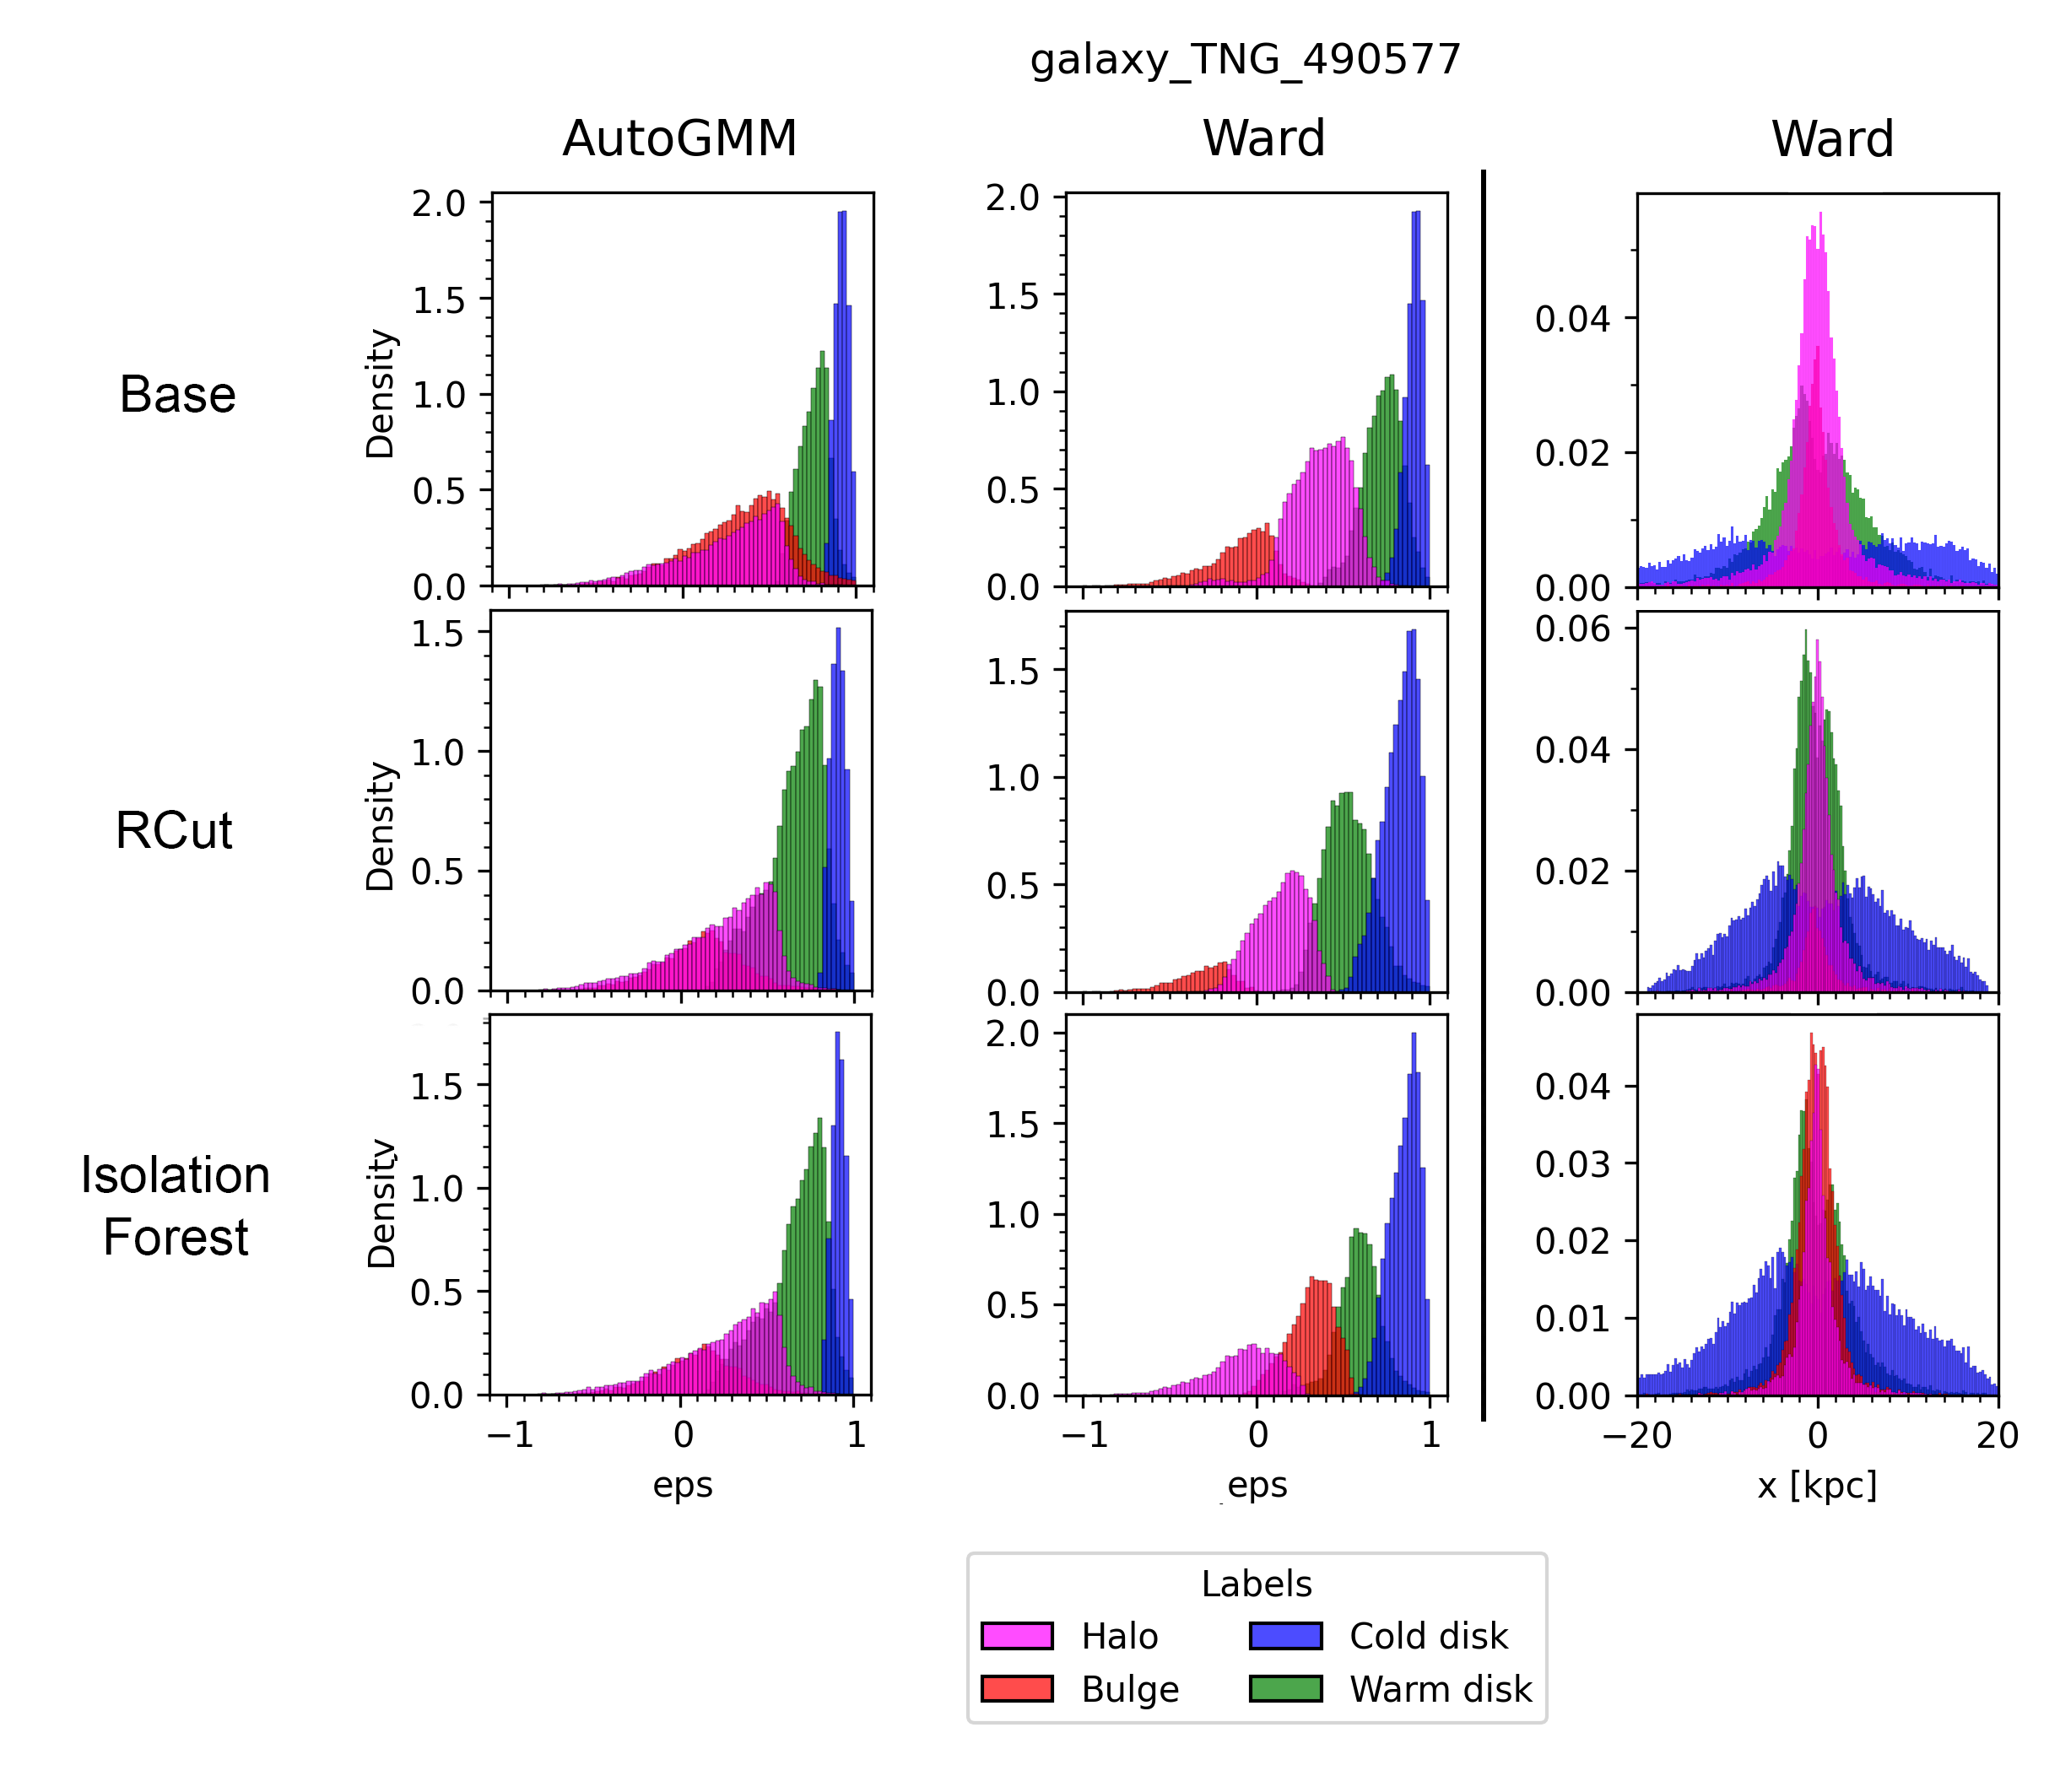
\includegraphics[width=12cm]{clustering jerarquico/figures/AGMM - galaxy_TNG_490577 - complete.png}
    \caption{Comparación de histogramas en espacio circular y real entre \gls{AGMM} y \gls{HC} sin tratamiento de outliers, luego aplicando \gls{RCUT}, y luego aplicando \gls{IF} sobre la galaxia \textit{galaxy\_TNG\_490577}.} 
    \label{fig:AGMM490577Complete}
\end{figure}

Sin embargo, dado que la cantidad de clusters a buscar es establecida automáticamente por lo encontrado por \gls{AGMM}, remover partículas estelares con métodos de eliminación de outliers resulta en la variabilidad de dicha cardinalidad, ya que el conjunto de datos con los cuales \gls{AGMM} trabaja es diferente, resultando así en potencialmente un conjunto de componentes diferentes. Esto puede observarse en la Fig~\ref{fig:AGMMDifferentComponentsFound}.

\begin{figure}
    \centering
    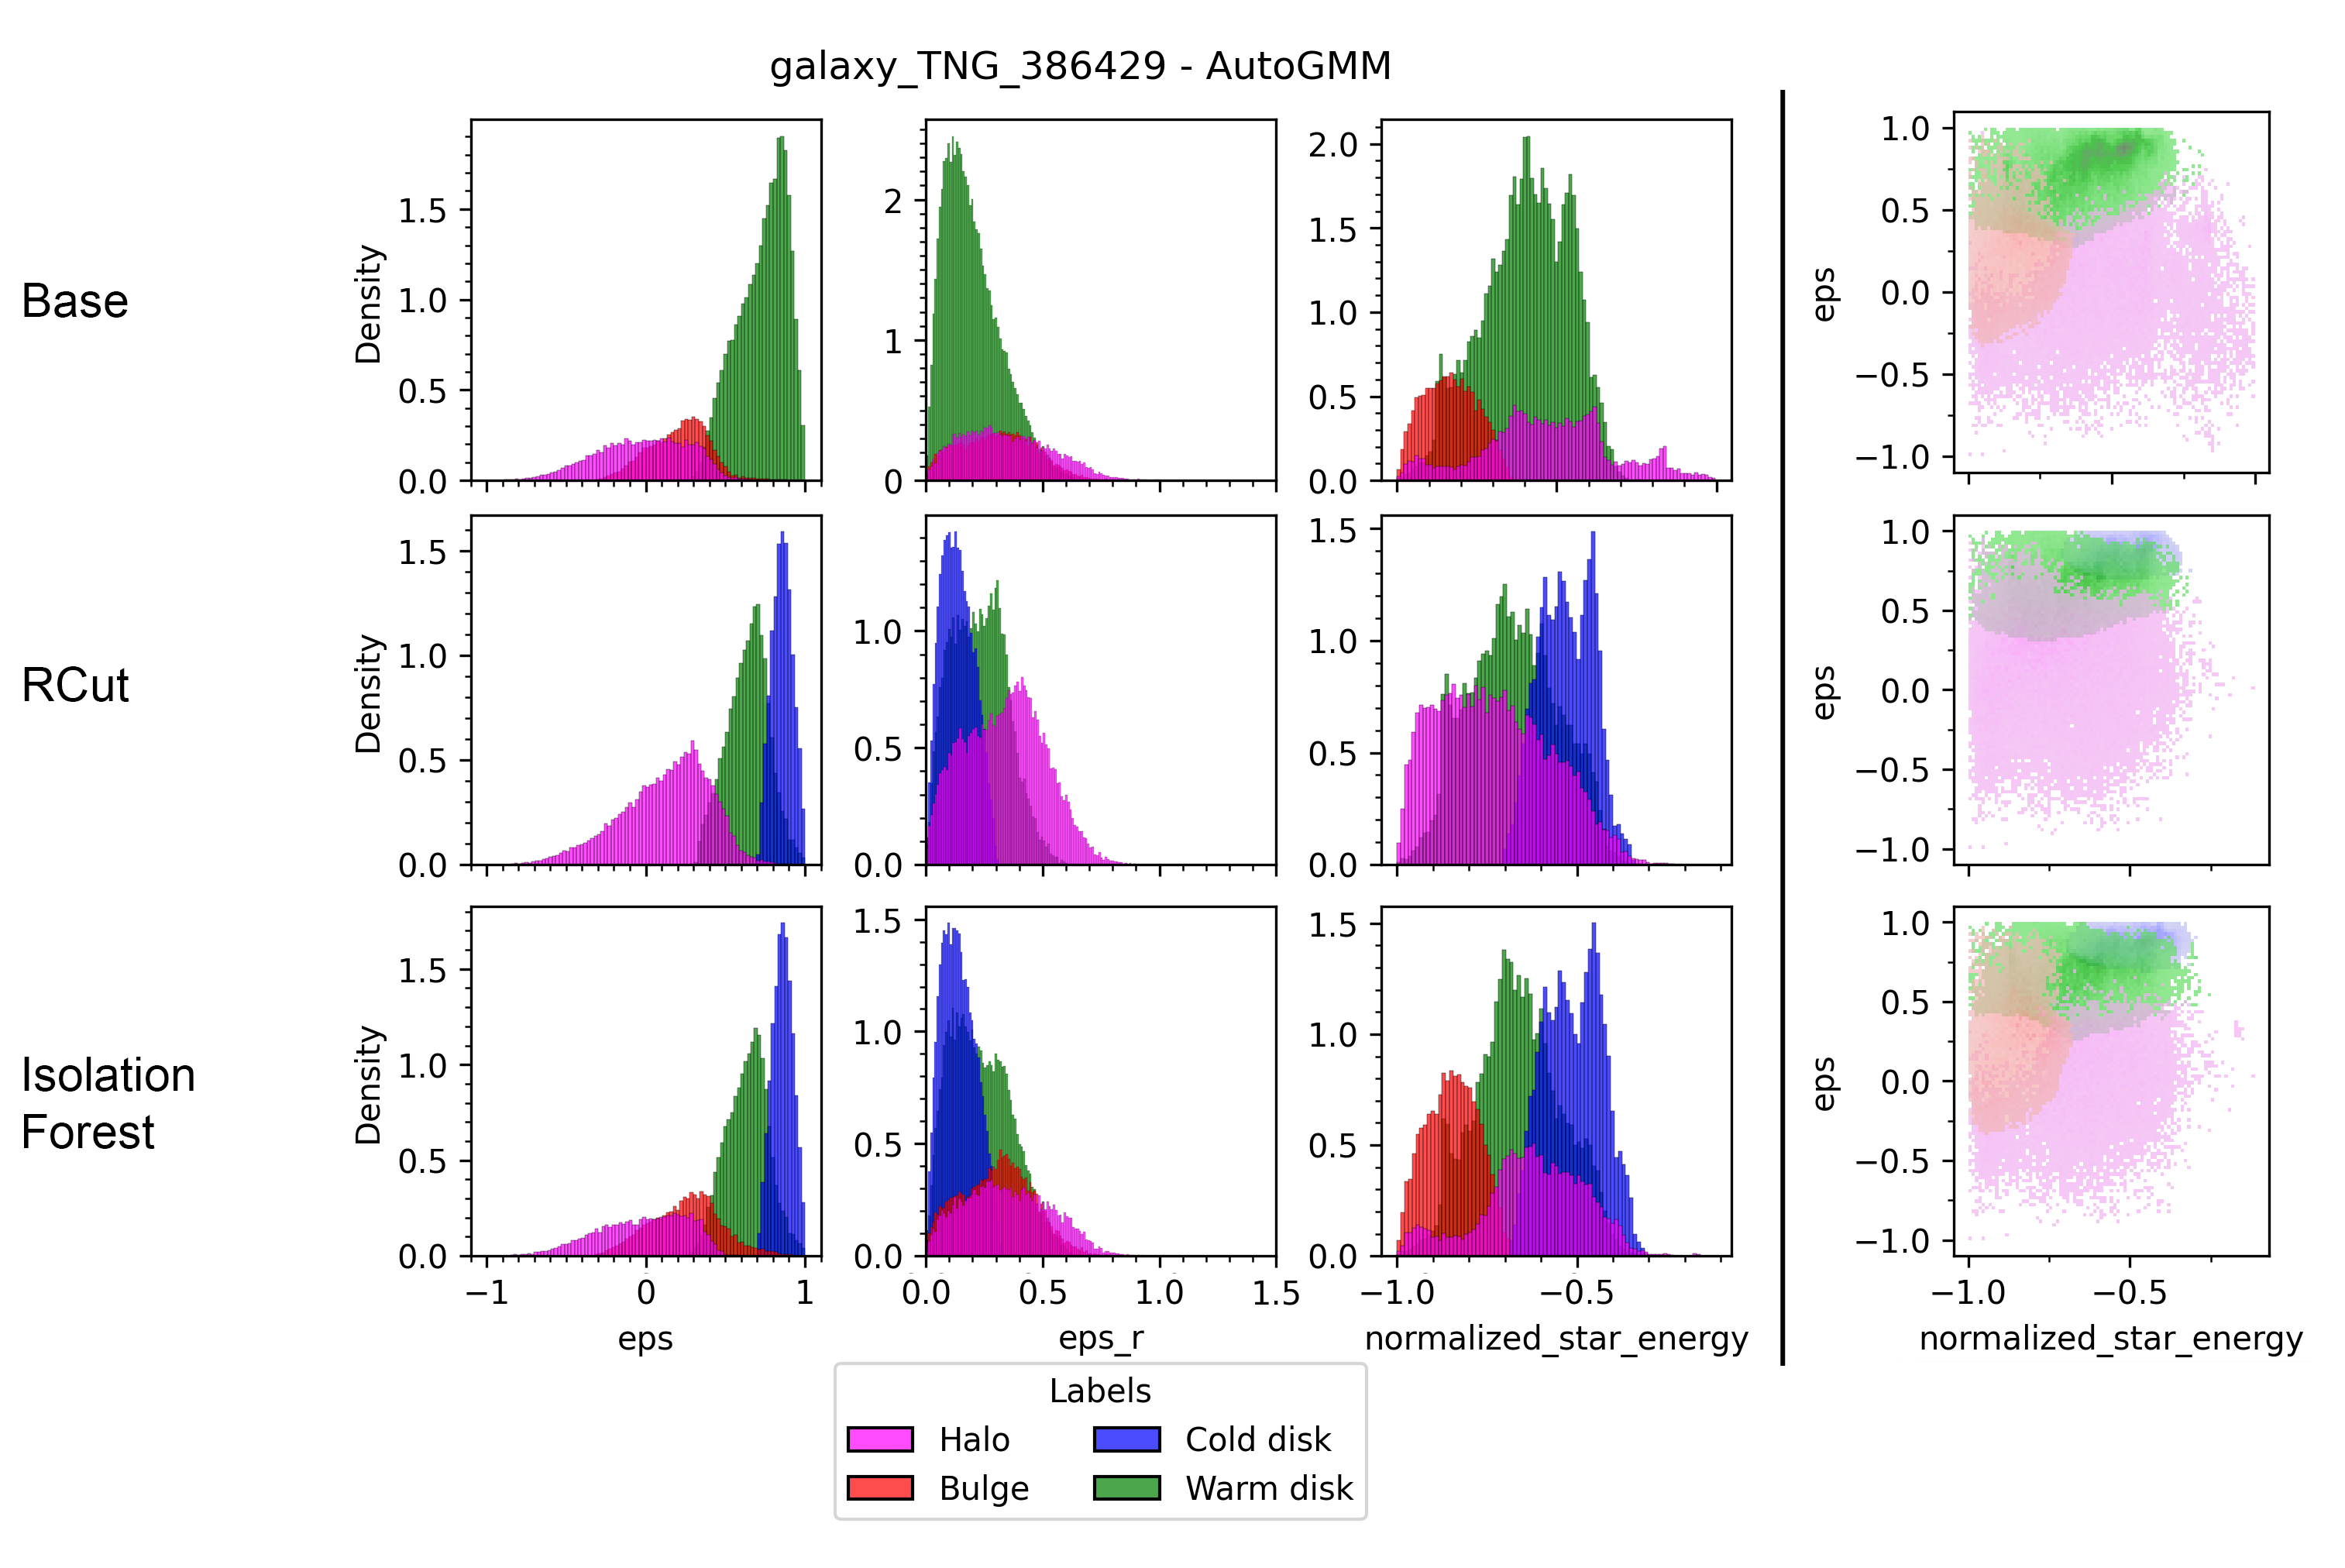
\includegraphics[width=12cm]{clustering jerarquico/figures/AGMM - different components found.png}
    \caption{Comparación de como \gls{AGMM} obtiene diferente cardinalidad de componentes al correr diferentes métodos para remover outliers sobre la galaxia \textit{TNG\_389511}.} 
    \label{fig:AGMMDifferentComponentsFound}
\end{figure}

Pueden verse las galaxias cuya cardinalidad de componentes no fue alterada al remover outliers en el Apéndice~\ref{appendix}, pero dado que éstas son menos de la mitad de nuestro dataset, y que no hay una clara mejora en los resultados obtenidos al aplicar \gls{HC} al remover outliers sobre éstas (como bien lo ejemplifica la Fig~\ref{fig:AGMM490577Complete} y la Fig~\ref{fig:NcomponentesRotationCurve}), no podemos concluir que remover outliers con \gls{RCUT} o \gls{IF} sea beneficioso para la clusterización obtenida con \gls{HC} al buscar más de dos componentes.

\begin{figure}
    \centering
    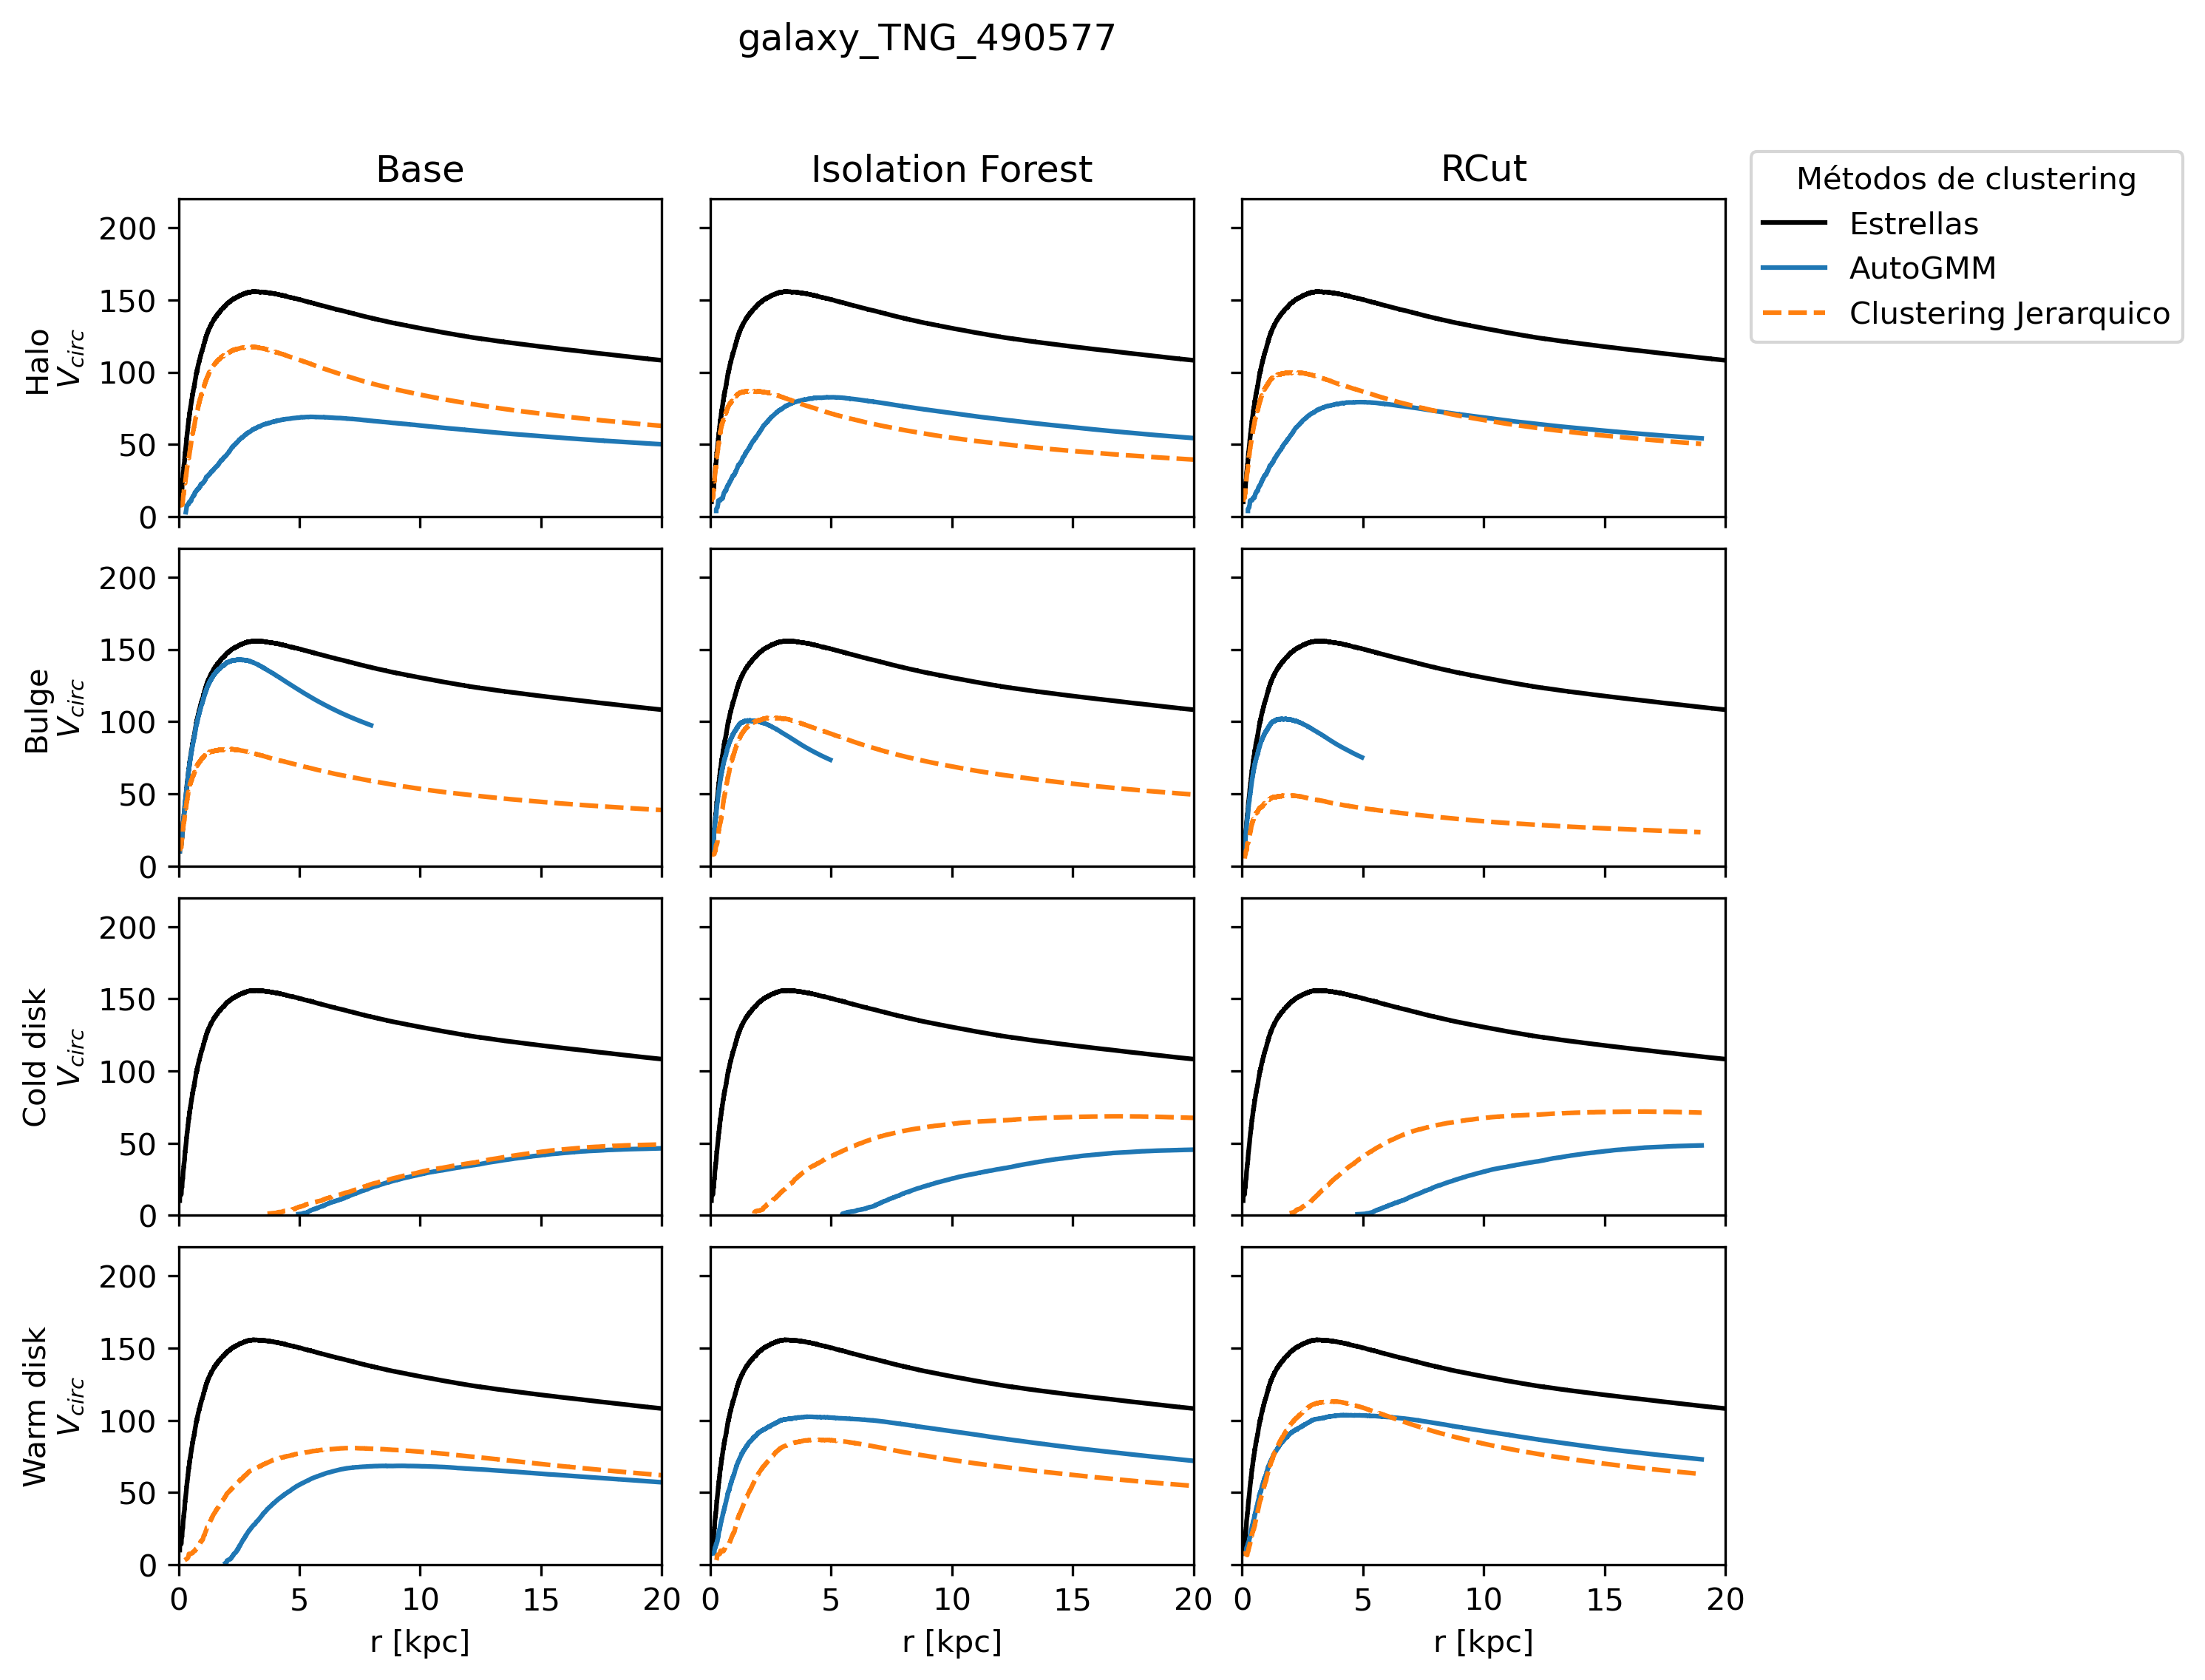
\includegraphics[width=11cm]{clustering jerarquico/figures/galaxy_TNG_490577 - AutoGMM - circ_velocity}
    \caption{Curva de rotación sobre los resultados obtenidos con \gls{AGMM} y \gls{HC} sobre la galaxia \textit{galaxy\_TNG\_490577}, utilizando diferentes métodos de eliminación de outliers.}
    \label{fig:NcomponentesRotationCurve}
\end{figure}
